\documentclass[oribibl]{llncs}
\pagestyle{headings} %page numbers
\usepackage{makeidx}  % allows for indexgeneration
\usepackage[utf8]{inputenc}
\usepackage[table,xcdraw]{xcolor}
\usepackage{multirow}
\usepackage{pdfpages}
\usepackage{float}
\usepackage{enumitem}
\usepackage[T1]{fontenc} % Fixed missing font warning for \maketitle
\usepackage{url}
\usepackage{todonotes} % remove later - this is for TODO notes
%\usepackage{amsmath,amssymb}  We don't use this?
\usepackage{url}
\usepackage{alltt}

% \hypersetup{%
%   citecolor=black
% }

\bibliographystyle{plain}

\begin{document}
\mainmatter{}
\title{Touch Based, Visual Syntax for Idris}
\author{Nicolai Dahl Blicher-Petersen \and Christian Harrington \\
\email{\{ndbl, cnha\}@itu.dk}}
\institute{IT University of Copenhagen, Rued Langgaards Vej 7, 2300 Copenhagen S, Denmark}

\maketitle

\begin{abstract}
In dependently typed programming languages, the type system can help provide powerful tool support, allowing for a faster and more
convenient way of programming e.g. by means of automatic case splitting and code-inference. Touch-based programming interfaces are often
cumbersome to use due to the heavy reliance on the virtual keyboard, so
minimizing its use could potentially benefit the programmer tremendously.

In this report we investigate the potential of the dependently typed
programming language, Idris, in the field of touch-based programming.
We propose a more visual, high-level syntax for Idris and describe our prototype of a structured editor
that supports this syntax and runs on the Apple iPad.

Through a thorough analysis of existing solutions, usability tests, and
heuristics evaluations, we evaluate our prototype and present a road map for
future work on the editor.

\todo{Insert what we conclude}

\keywords{VPL, Idris, Structured Editor, Usability}
\end{abstract}
%!TEX root = ../Touch Based Idris.tex
\chapter{Introduction}
\label{sec:Introduction}

Currently, there is no widespread visual programming solution, although the field has been explored for half a century. In the last few years touch-based interfaces, in the form of smart phones and tablets, have proliferated. These devices often rely on virtual keyboards for text-input, which can be cumbersome to use, especially when programming. 

Idris is ``a general purpose functional language with dependent types''\,\cite{brady2013idris}. The expressive nature of the Idris type system makes advanced tool-support possible, such as automatically generating pattern matching on the different possible constructors for a term, or even filling out a term automatically. In these cases, the compiler will be able to fill in the code automatically when asked to. Idris has a strong core language that can be extended with a higher level syntax as long as it can be translated back to the core language.

The goal of this project is to explore how best to present and interact with a visual syntax on a touch-based device, using the advanced tool support afforded by Idris to minimize the use of the virtual keyboard.

To accomplish this, we will first study existing solutions for touch-based and graphical programming, and aim to identify and define their usability shortcomings by using existing usability theories. Secondly, we will classify these usability issues to provide an overview of successful approaches as well as pitfalls. 
\todo{Is classify the right word here? Are we promising too much?}

With the knowledge we have gained from these activities, we will present a set of requirements for our solutions and propose a new visual, high-level syntax for Idris that adheres to these. We will then iteratively usability test and develop a simple prototype application for iOS on the Apple iPad, allowing a user to manipulate this visual syntax using touch gestures. We will also examine the practicalities of adding support for this high-level graphical syntax to the Idris compiler, so programs written in the graphical syntax can be executed.

To evaluate our solution, we will perform a heuristic evaluation with reference to our requirements. Finally, we will produce a plan for future empirical usability tests that will serve as basis for the further development of the prototype.


\section{Overview}
Section \ref{sec:DependentTypes} gives an overview of Idris and some of its
most relevant language features. Section \ref{sec:Analysis} analyses a
wide range of existing visual, touch-based, or structured languages and Section
\ref{sec:GoalsAndRequirements} leverages this analysis to present a list of
goals and requirements for our solution design. The initial design together with the first usability
iteration is presented in Section \ref{sec:InitialDesign}. Section \ref{sec:Architecture}
supplies a discussion of our software architecture and forms the basis for the
implementation section (\ref{sec:Implementation}), where our prototype is
described together with a second usability iteration. Finally, Section \ref{sec:Evaluation}
evaluates our prototype and provides a road map for further development, Section \ref{sec:Reflection} reflects
upon our process, and Section \ref{sec:Conclusion} concludes the report.





%!TEX root = ../Touch Based Idris.tex
\section{Background}
\label{sec:Background}
\subsection{Dependent Types}
In many programming languages, such as Java or Haskell, a type can depend on another type, such as \texttt{ArrayList<A>} in Java, or \texttt{[a]} in Haskell. By suppling a concrete type, we can say that a collection only holds this specific type of values, e.g. \texttt{ArrayList<String>} or \texttt{[String]}. But in a programming language with dependent types, it is possible to go further. With dependent types, a type can be dependent on \emph{values} as well as types. This allows for increased expressiveness in the type system, which can be used for ensuring correctness, conducting proofs, and improving tool support. For this project, it is the last point we will focus on. Dependent types have been implemented in several programming languages, such as Coq\todo{Ref}, Agda\todo{Ref}, and Idris, which we will examine next.

\subsection{Idris}
\label{subsec:Idris}
Idris is a dependently typed programming language, initially developed by Edwin Brady~\cite{Idris}. The syntax is heavily inspired by Haskell. Let us start by looking at a simple example. In Figure~\ref{fig:nat}, a data type representing the natural numbers is defined. It consists of two constructs \texttt{Z}, representing zero, and \texttt{S~n}, representing the successor of the natural number \texttt{n}.

\begin{figure}
\begin{alltt}
data Nat : Type where
  Z : Nat
  S : Nat \(\to\) Nat
\end{alltt}
\caption{The natural number data type.}
\label{fig:nat}
\end{figure}

The definition for \texttt{Nat} looks similar to how it would look in Haskell. Let us move to a slightly more complex example, where we make use of dependent types. In Figure~\ref{fig:vect}, the dependent vector, \texttt{Vect: Nat $\to$ Type $\to$ Type} is defined. This type takes two arguments: a \texttt{Nat}, \texttt{n}, describing the length of the vector, and a \texttt{Type}, \texttt{a}, specifying the type of the elements it contains.

\begin{figure}
\begin{alltt}
data Vect : Nat \(\to\) Type \(\to\) Type where
  Nil  : Vect Z a
  (::) : a \(\to\) Vect k a \(\to\) Vect (S k) a
\end{alltt}
\caption{The vector data type.}
\label{fig:vect}
\end{figure}

The first construct, \texttt{Nil}, tells us that the empty vector always has a length of \texttt{Z}, or zero. The second constructor, \texttt{(::)} or cons, takes a new element of type \texttt{a}, and prepends it to a vector holding elements of type \texttt{a}. The length of the resulting vector is increased by one compared to the previous vector. We say the vector is parameterized by the type \texttt{a}, as it is the same in both constructors. However, the length of the list, specified by the natural number \texttt{n}, is different in each constructor, so we say the vectors is a family of data types \texttt{indexed} by the natural numbers.

But why record the length of the vector in its type? How does this help us? A simple example of how this can be useful can be seen in the \texttt{zip} function, shown in Figure~\ref{fig:zip}.

\begin{figure}
\begin{alltt}
zip : Vect n a \(\to\) Vect n b \(\to\) Vect n (a, b)
zip Nil       Nil       = Nil
zip (x :: xs) (y :: ys) = (x, y) :: zip xs ys
\end{alltt}
\caption{Zip function for vectors in Idris.}
\label{fig:zip}
\end{figure}

The \texttt{zip} function takes two arguments. Each argument is a vector of the same length \texttt{n}. \texttt{n}, \texttt{a}, and \texttt{b} are inferred implicitly from their context. These arguments could also be explicitly declared as implicit by surrounding them with curly braces: \texttt{\{n:~Nat\}~$\to$ \{a:~Type\}~$\to$ \{b:~Type\}~$\to$ Vect~n~a~$\to$ Vect~n~b~$\to$ Vect~n~(a,b)} The function zips these two vectors together, producing a vector of the same length, containing tuples \texttt{(a, b)} of the values from the input vectors. If one tries to compile a program that attempts to zip two vectors of different lengths, the type checker will report it as an error, as opposed to failing at runtime. Notice how it is unnecessary to match on the cases where one vector has elements while the other is empty. This situation is impossible, due to the types. In fact, matching on this case is ill-typed, as \texttt{Z} and \texttt{S~n} cannot unify.\todo{Should we mention dependent pairs and the with-rule, when we don't support them?} For our final example, let us look at the \texttt{filter} function in Figure\ref{fig:filter}.

\begin{figure}
\begin{alltt}
filter : (a \(\to\) Bool) \(\to\) Vect n a \(\to\) (p ** Vect p a)
filter p [] = (_ ** [])
filter p (x::xs) with (filter p xs)
  | (_ ** tail) =
    if p x then (_ ** x::tail) else (_ ** tail)
\end{alltt}
\caption{Filter function for vectors in Idris.}
\label{fig:filter}
\end{figure}

The \texttt{filter} function uses two constructs that we have not seen so far, dependent pairs and the with rule. Dependent pairs let us specify a type that is dependent on another value. In \texttt{filter}, we do not know beforehand what length the resulting vector will have, so instead we return a dependent pair, where the first element is the length, and the second element is a \texttt{Vect} of that length. Not knowing the length is also a problem in the cons case of \texttt{filter}. If the head of the \texttt{Vect} passes the predicate \texttt{p}, we want to cons the tail of the \texttt{Vect} onto the head. But since we do not know what the length of \texttt{filter p xs} is beforehand (as it depends on how many elements passes the predicate \texttt{p}), we cannot construct the type for the resulting vector. But by using the \texttt{with} keyword, we can pattern match on the result of \texttt{filter p xs}. We know the length of \texttt{tail}, since we have filtered it already, so we can construct the resulting \texttt{Vect} without any problems. The underscores (eg. \texttt{(\_ ** tail)}) tell Idris to infer the value.
%!TEX root = ../Touch Based Idris.tex
\section{Analysis of Visual and Touch Based Solutions}
\label{sec:Analysis}

In this section, we evaluate a range of visual and/or touch based programming interfaces and languages. It is the goal of this phase to be able to compile a list of desirable and undesirable features for our IdrisTouch editor.

\subsection{Investigation Scope}
The amount of touch-based and/or visual programming languages and editors that have already been developed is quite large as can be seen from Eric Hosick's list.\,\cite{hosick2014} For this very reason it was important for us to define which types of existing solutions that are of interest to us.

As we’re designing a visual touch-based syntax for the programming language Idris, we can define our target group to users that are familiar with dependently typed languages. Plenty of experiments with visual languages for educational purposes have been conducted (see Scratch section) (Pane et al., A. Myers, Green), so we should only take more experienced programmers into consideration when designing the user experience.

As Idris is general purpose we will not be investigating domain specific languages/platforms unless elements of their syntax or IDE has potential of working with general purpose languages.

There are many visual workflow editors that basically use a collection of boxes and arrows to visualize state and actions. Author and Author \todo{insert ref} argue that purely visual languages like these do not scale well. Our focus has thus moved away from purely visual workflow languages to languages that only partially rely on visual syntax.

Still, with these limiting factors there are too many candidate solutions for us to analyze and evaluate them all. The following analysis consists of a selection of the available solutions that we found most relevant to our study and mainly applies the heuristic evaluation technique by Nielsen\,\cite{nielsen1990heuristic}. Such an evaluation can give an idea of possible usability issues but I will not help discover them all. This suits our purpose, as it is our mission to get an overview of the major pitfalls as well as what generally works well when designing our solution. Furthermore, we are pursuing an entirely new type of touch-based, visual, and structured interface instead of bettering an existing one so analyzing a few existing solutions in depth does not make sense.

The thoroughness of our analyses also depend on something as practical as whether we have been able to install the tool/language on our machines. Some of the solutions in question are old and experimental only. In some cases the only thing available are conceptual descriptions by the creators.

\subsection{Visual Programming Languages}
We will be investigating two Visual Programming Language (VPL) as well as Epigrams hybrid approach in this section.

\subsubsection{Labview}

Labview is a development environment featuring the VPL, G, which is designed for dataflow programming and uses the popular ``boxes and wires'' abstraction, with boxes performing various functions, and wires leading data between the boxes. Labview also lets users combine simple widgets to build GUI programs, using the G language for logic. It is widely used in the scientific community, especially to work with data collected from sensors.

Labview is often referenced in the literature of VPLs \todo{insert a couple of references}, so even though it is domain specific we find it interesting as a starting point for our investigation.

While complex programs in G can be initially overwhelming to even experienced programmers, Whitley and Blackwell \todo{WHITLEY AND ALAN F. BLACKWELL (ref)} show that seasoned Labview programmers prefer the visual syntax to a textual one.

It is interesting how Green and Petre \todo{(ref)} give Labview an overall positive response when evaluating it through the cognitive dimensions framework, it would almost certainly be viewed more negatively using the Physics of Notation framework\todo{ref}. Like UML, G does not make use of many of the principles, such as Visual Expressiveness, Perceptual Discriminability and Complexity Management.

\paragraph{Takeaways}
\begin{enumerate}
	\item One interpretation of Whitley and Blackwell's findings \todo{WHITLEY AND ALAN F. BLACKWELL (ref)} is that although Labview can be hard for programmers not used to the visual syntax, the higher learning curve pays off in the long run.
	\item The fact that Labview does not make use of the various principles of physical notation might help explain why newcomers find it daunting.
	\item The ``boxes and wires'' approach is good at indicating structure and could maybe be transfered to a more general purpose language representation such as IdrisTouch.
\end{enumerate}


\subsubsection{Scratch}
Scratch is a visual programming language designed to be easy for beginners to use, facilitating the development of simple audio/visual programs. It is implemented as a web app, and features built-in tutorials, tips and help.
The language is built around a scene containing sprites. A scene can have multiple sprites, and each sprite can be governed by multiple scripts written in the Scratch visual language. The language itself consists of blocks of different shapes, colors and sizes. Scratch does not use the dataflow paradigm, as Labview does. Instead, one programs by snapping blocks together. The blocks have different shapes, and only complementing shapes can be put together (think of puzzle pieces). Color is used to describe different types of blocks.

The user interface itself is a bit cluttered, and it is not immediately clear how the three main areas (scene, sprites, and scripts) interact. Once this has been discovered, however, it is reasonably easy to use. 

A wide range of solutions based on or similar to Scratch have been made over the years\,\cite{hosick2014}, but one is, in particular, interesting to us as it is a port of Scratch to the Apple iPad. It is called Hopscotch\,\cite{hopscotch} and generally does exactly what Scratch does just by incorporating two types of simple touch gestures.

The most interesting part of Scratch is the visual language, which will be evaluated using the principles from The Physics of Notation \todo{ref} instead of Nielsen's Usability Heuristics as it is more fitting in this particular case.

\paragraph{Principle of Semiotic Clarity}
There is a clear onscreen representation of every abstract element, and only that one representation.

\paragraph{Principle of Perceptual Discriminability}
Use of different colors for different types of elements (control structures, data management, input), along with different shapes for showing which elements can be combined makes it very easy to discriminate between different components.

\paragraph{Principle of Semantic Transparency}
While many elements are too abstract to have an obvious visual representation (what does a variable ``look like''?), symbols are used in a semantically immediate way in some places, such as an arrow pointing back to the start of a loop. 

\paragraph{Principle of Complexity Management}
Complexity management is a problem for Scratch, as there does not seem to be a way to define new functions. This means functions can become very long and unwieldy. The general discussion if visual programming languages have scalability has been explored in depth by Green and Petre \cite{green1992visual}.

\paragraph{Principle of Cognitive Integration}
Scripts cannot access anything from other scripts, so this is not possible to implement. \todo{elaborate}

\paragraph{Principle of Visual Expressiveness}
Uses shape, color, and position to convey meaning. \todo{elaborate}

\paragraph{Principle of Cognitive Fit}
Does not have different representations for different tasks, as there is only one task. The ``block'' nature of Scratch further means it is not possible to create invalid programs, only elements that make sense can snap together, which is very valuable to beginners.

\paragraph{Other dimensions}
Scratch makes no or very little use of the principles of Dual Coding and Graphic Economy.

\paragraph{Takeaways}
\begin{enumerate}
	\item When designing a visual syntax, making it visually obvious which elements go together greatly increases the ease of learning.
	\item Using colors and shapes to differentiate elements is very important in a visual language.
	\item Complexity management is hard with visual languages\,\cite{green1992visual}. It should be easy to define functions. 
	\item Composability should be an important goal.\todo{why?}
	\item Use all the aspects of visual expressiveness when designing a visual language, e.g. shape, color, texture, position, etc.
\end{enumerate}

\subsubsection{Epigram}
The Epigram language is a functional and dependently typed language made by Conor McBride, which aimed to let the programmer create compiler certified proofs using intuitionistic logic. It is not really a visual programming language, but it has been put in this category as the syntax of the data type specification is interesting. In Epigram, defining data is done in a more visual way than newer dependently typed programs. This is done by imitating the standard form for writing inference rules. The definition of e.g. a data type is split into three lines and its 2D syntax almost resembles ASCII art. 

While it has been impossible to get a version of Epigram working for any sort of test we are interested in how this way of expressing data types could benefit the user in a more structured editor that does not require the user to maintain ASCII art but still displays the program in a more visual way.

\subsubsection{Takeaways}
\begin{enumerate}
	\item Imitating the standard form for writing data types seems to be intuitive and goes well with Nielsen’s ``Match between system and the real world''-heuristic.
\end{enumerate}

\paragraph{}

There is a tendency for visual programming languages to be domain specific and such it is natural that a high-level syntax for a general purpose language like Idris is less visual. We will, however, investigate Epigram's way of defining and presenting data types.

\subsection{Touch-based Programming Languages}


\subsubsection{CodeToGo}
CodeToGo claims to be the first app for iOS in which you can write and run code in your favorite language\todo{ref}. It is backed by the ideone.com website\todo{ref} that evaluates the code, when the user presses “Run”. The app provides shortcuts for the most commonly used characters and even lets you customize which ones to have easiest access to in which language. The usability considerations stop here though. CodeToGo does not take advantage of the touch based interface but tries to overcome it. While there is syntax highlighting there is no code completion or static checking, which quickly makes programming a cumbersome task.

The most severe usability problem for CodeToGo is the low degree to which the user is able to recover from errors. If you have a syntax error in your code you will get a standard console compile error from the ideone.com server. This error contains the line number where your program failed, but when you dismiss the error you will have to remember this line number and manually count your way down to the line where the mistake was, as the editor does not display line numbers\,\cite{nielsen1990heuristic}.

The editor only has the aforementioned character selector as an accelerator for advanced users. Other than that there are no ways for users to improve when using the tool other than to learn to type faster on an iPad\,\cite{nielsen1990heuristic}.

Nielsen \todo{year} recommends that you follow the iOS platform standards so that the user does not have to put too much effort into learning how to use each app in a special way. Nielsen also recommends having undo support. CodeToGo does have undo support and follows the standard way of iOS, which is to shake the device. One could argue that shaking their iPad is not the most elegant way of allowing programmers to undo their typing, so in this case following the standards is not necessarily the best way to go for a mobile programming interface.

\paragraph{Takeaways}
\begin{enumerate}
	\item Do not assume that a virtual keyboard is as usable as a physical one\,\cite{nielsen2013mobile}. The touch interface has potential if you design your user experience to take advantage of it, but if you chose to ignore its potential/limitations you will have lower usability.
	\item You need accelerators for users to become faster and more comfortable with the interface. An accelerator could, for example, be auto completion and/or static checking.
	\item Undo support is essential for usability\,\cite{nielsen1990heuristic}, but if shaking the device is the right input method is questionable.
\end{enumerate}

\subsubsection{Textastic}

Like CodeToGo, Textastic aims to be a general purpose programming editor, and as such supports many popular programming languages. Unlike CodeToGo, however, it does not support any way to run your code (besides manually copying your program to a computer and running the code there). Textastic is interesting due to an interface component that is not seen in CodeToGo.

Textastic uses a smart shortcut bar to allow quick access to commonly used characters, that would otherwise be hard to get to with the virtual keyboard.\todo{insert image} The biggest problem with Textastic is that you have no way of knowing whether your code will run or not.\todo{ref 10 heuristics. Specifically, user feedback} On a computer, this would not be as big of a problem, in fact many programming editors do not touch on the semantics of the language they are editing, instead they rely on other software to run the code. This is much harder on a device such as an iPad, where multitasking is not as prevalent. The text editing interface is very reminiscent of none-touch GUI text editors, such as TextMate or Sublime Text. 

\paragraph{Takeaways}
\begin{enumerate}
	\item Even in our IdrisTouch interface there will be a need for inputting special characters, and the solution Textastic has come up with is the most intuitive we have seen.
	\item It is not enough to have a good editing interface, if such a basic issue as running your code is unaddressed.
\end{enumerate}



\subsubsection{Raskell}

Raskell is a Haskell editor for the iPad. It is based on the Hugs implementation of Haskell 98, and includes the ability to interpret your programs locally. The text editor itself is inspired by Vi, featuring many of the same keyboard commands. When you have written your program, you can load it into the interpreter, which gives you a REPL, letting you test out your program. Raskell supports syntax highlighting for Haskell, and features most libraries for Hugs, but does not have auto completion.

The text editing itself is fine, but a lack of autocomplete and snippets mean you will be using the virtual keyboard a lot. The error messages when running your code obscure the code, meaning you have to read and memorize the error before trying to fix it, although it also features inline error messages while programming. The REPL is extremely useful for trying out parts of your program 

While otherwise a good experience, Raskell does nothing to reduce use of the virtual keyboard, which can be tedious to use for longer periods.

\paragraph{}

Recap here what we like the most from the touch based


\subsection{Structured Programming Languages}



\subsubsection{Lisping}

Using the Scheme dialect of LISP you can program and execute code right on your iPad with Lisping. The idea is to take advantage of the close proximity between the abstract syntax tree and source syntax of LISP to edit code in a structured way. So you are actually manipulating the abstract syntax tree almost directly instead of having to type in every single character of every single line. While other iPad solutions run code on an external server, Lisping runs locally using a Scheme interpreter written in C, called TinyScheme.

Lisping has been written with usability in mind as it is stated on the website: 

“Textviews and virtual keyboards aren't the only option for coding on iOS. Editing source code character by character is a concept wedded to the keyboard and it is not necessarily the best option for a device with no keyboard.” [http://slidetocode.com/lisping/]

We’re fairly experienced programmers with only little knowledge of the Scheme language and it’s syntax and we had a hard time using Lisping. The underlying TinyScheme interpreter most often gave us “Error Unknown” compiler messages even though we were writing examples straight from the Scheme website. Not being able to pinpoint what was syntactically wrong with the written code was a major issue.

The editor supports a range of touch gestures that are not immediately obvious to the user. You have to open the Lisping guide in the upper right corner and read through 6 pages of a pdf document to familiarize yourself with these gestures, which has low memorability.

There are also several buttons on the bottom of the UI. These are all icons and except for the delete and edit ones, they have no standard meaning in iOS or are used differently from the standard meaning. The undo button is e.g. a backwards-pointing triangle which could be interpreted to mean “Back” in iOS. Given the fact that I have no chance of remembering all these non-standard icons, they clearly violate the “Recognition rather than recall” and “Consistency and standards” usability guidelines presented by Nielsen (year). 

Furthermore, these icons are all located close to each other and a whole screen length away from where my attention is supposed to be when I’m programming - that is, on the code. All but two of the actions that these icons allow the user to do can be done with various gestures performed on the source code, which is a failed attempt on providing accelerators for the expert user.

The problem with these gestures is that they are uncomfortable. To select an expression to edit or run in the REPL, the user must “reverse pinch” the text. This is a non-standard way of highlighting text in iOS and it feels very awkward and unresponsive not to mention that it gets painful to do after you’ve done it 3-4 times. The font size of the code should also be larger, as it is difficult to hit the intended buttons.

The final usability problem we discovered with Lisping was the amount of + buttons inlined in the code. These buttons are supposed to indicate that an expression can be added there, but all they really do is make the code harder to read. 

\paragraph{Takeaways}
\begin{enumerate}
	\item The error messages from the compiler/interpreter should indicate where in the code the syntax errors have occurred. Simply presenting “Unknown Error” is frustrating for the user.
	\item It should not be necessary to add a pdf documents with instructions to how the gestures and buttons work. It should be immediately recognized by the user because it is all presented according to the platform standards. Don’t get “too creative” with gestures and button icons.
	\item Littering a structured editor with + (add) buttons, to indicate that expressions can be added at these positions, is not a good idea if you want a proper overview. While a good alternative for this solution is hard to come up with we should try to design a different way.
\end{enumerate}



\subsubsection{Eastwest}
Even though Eastwest is basically an experiment we find it very interesting. It is a structured editor for a functional language that allows the user to “fill in holes” i.e. fulfill goals of a program from a context. The context appears right under the goal and thus works as a well-placed autocompletion tool. We have been unable to complete a usability test of Eastwest, as we were unable to install it on our computers. Several videos are available, though, and it is interesting to see how functional data types are being defined and functions are being built in a structured way.

\paragraph{Takeaways}
\begin{enumerate}
	\item Having a context close to the goal makes for quick and easy access. The better that context is at guessing the right thing for the goal, the faster the tool will seem.
	\item Functional languages seem to work well in a structured editor.
\end{enumerate}


\subsubsection{TouchDevelop}

TouchDevelop allows developers to make touch and accelerometer enabled games for any device with a web browser by providing a web app. It is generally meant as a way of getting young people interested in programming, and the language has been specially designed for this purpose and works hand in hand with the development platform to provide a good experience for touch devices.

TouchDevelop is not general purpose but focuses on creating simple 2D games. This means that the user gets a lot of standard game concepts built into whatever program he’s writing. This is evident from the context that is being updated as you type in the bottom of the screen. This basically means that you rarely have to type characters into the editor as you don’t have to define new methods (actions). Variable names are automatically generated at the push of a button.

The first thing you notice as an experienced programmer is how the TouchDevelop language looks like modern imperative languages like C\# and Java, and this recognizability enabled me to get started with the platform right away. To educate new users there is a long tutorial that guides you through your first game. This tutorial makes the language seem very structured but in fact it is as easy to make syntactical error as in any other imperative language.

Even though TouchDevelop works on all touch devices that has a web browser it is not really optimized for other gestures than the standard single tap gesture that works on all platforms.

To fit more code on the screen and create a better overview, TouchDevelop uses a rather small font for the code you write. When you tap the line of code you wish to edit, that statement is enlarged and you can relatively easily move the cursor around. Additionally, buttons appear to insert new lines above and below the selected segment. This design is minimalistic and controls only show up when you need them.

The context that is presented to the user to select method calls and objects from is convenient when it presents you with just what you needed, but in most cases you find yourself struggling to find just that. This is due to the nature of object oriented systems. When filling out a “hole” in the program the type system cannot narrow down the possibilities, as any object could potentially allow the user to create the right type. This seems to be a problem for us as novice users, as the vast number of elements in the context at any given time slows down the speed of which we’re programming.

The “feel” of TouchDevelop suffers from the fact that it is a web app written with no specific system in mind. The biggest annoyance is when you want to move around the cursor. This is clumsy on the iPad and often requires that you use buttons.

\paragraph{Takeaways}
\begin{enumerate}
	\item To have a contextual overview can speed up the tasks.
	\item 
\end{enumerate}

The type system of an object oriented programming language is not ideal if you want to expose a context for the user to pick from. The type system simply can’t narrow down the possibilities efficiently.
Using a smaller font for code that is not in focus is a clever way to create a better overview for the user.
If you want a nice native “feel” to an app, you should write it specifically for one platform.

\paragraph{}

Briefly tell why Idris is good for the structured approach


\subsection{Existing Solutions Overview}
Table \ref{table:existing_solutions_overview} gives an overview of the existing solutions and how we will be positioning our IdrisTouch solution compared to these. Our study indicates that touch gestures can be used as accelerators for super users, so we will have focus on implementing these where it makes sense. The strong type system of Idris allows us to make a more structured editor than most existing solutions. Lastly, it is our theory that we can represent Idris data types in a more visual way than what programmers are used to from the current concrete syntax.
	
% Please add the following required packages to your document preamble:
% \usepackage{multirow}
% \usepackage[table,xcdraw]{xcolor}
% If you use beamer only pass "xcolor=table" option, i.e. \documentclass[xcolor=table]{beamer}
\begin{table}[ht]
	\begin{tabular}{|l|l|l|l|l|}
	\hline
	                      & \textbf{Description}                                                                                              & \textbf{Touch-based}                                              & \textbf{Visual syntax}                          & \textbf{\begin{tabular}[c]{@{}l@{}}Stuctured \\ editor\end{tabular}} \\ \hline
	\textbf{CodeToGo}     &                                                                                                                   & \cellcolor[HTML]{B6D7A8}{\color[HTML]{9AFF99} }                   &                                                 &                                                                      \\ \cline{1-1}
	\textbf{Textastic}    & \multirow{-2}{*}{\begin{tabular}[c]{@{}l@{}}Textual iPad interface for \\ general purpose languages\end{tabular}} & \multirow{-2}{*}{\cellcolor[HTML]{B6D7A8}{\color[HTML]{9AFF99} }} & \multirow{-2}{*}{}                              & \multirow{-2}{*}{}                                                   \\ \hline
	\textbf{Epigram}      & \begin{tabular}[c]{@{}l@{}}Functional with Dependent \\ Types\end{tabular}                                        &                                                                   & \cellcolor[HTML]{6AA84F}                        &                                                                      \\ \hline
	\textbf{Raskell}      & Mobile Haskell                                                                                                    & \cellcolor[HTML]{B6D7A8}{\color[HTML]{9AFF99} }                   &                                                 &                                                                      \\ \hline
	\textbf{TouchDevelop} & \begin{tabular}[c]{@{}l@{}}Imperative language \\ running as a web app\end{tabular}                               & \cellcolor[HTML]{6AA84F}                                          &                                                 & \cellcolor[HTML]{B6D7A8}                                             \\ \hline
	\textbf{Lisping}      & Mobile Lisp                                                                                                       & \cellcolor[HTML]{6AA84F}                                          &                                                 & \cellcolor[HTML]{B6D7A8}                                             \\ \hline
	\textbf{Scratch}      & \begin{tabular}[c]{@{}l@{}}Beginner-friendly \\ programming by dragging \\ boxes\end{tabular}                     &                                                                   & \cellcolor[HTML]{274E13}{\color[HTML]{274E13} } & \cellcolor[HTML]{274E13}                                             \\ \hline
	\textbf{Eastwest}     & \begin{tabular}[c]{@{}l@{}}Functional programming \\ system with structured editor\end{tabular}                   &                                                                   &                                                 & \cellcolor[HTML]{274E13}                                             \\ \hline
	\textbf{IdrisTouch}   & Mobile Idris                                                                                                      & \cellcolor[HTML]{38761D}                                          & \cellcolor[HTML]{6AA84F}                        & \cellcolor[HTML]{38761D}                                             \\ \hline
	\end{tabular}

	\caption {Existing solutions overview}
	\label{table:existing_solutions_overview}

\end{table}

\subsection{Overall Takeaways}
In this section we have analyzed a range of existing solutions and for each reached a list of takeaways that we will be using to form our requirements for the IdrisTouch app.










%!TEX root = ../Touch Based Idris.tex 
\section{Goals and Requirements}
\label{sec:GoalsAndRequirements}

\subsection{Goals}
The overall goal of this project is to investigate how the features of the dependently typed language, Idris, can improve the touch-based programming experience. 
It is important to underline that the design we will propose is meant to compete with other touch-based editor designs, and not with traditional keyboard based editors.
In other words, we are not trying to revolutionize the way we program, instead we are trying to improve the programming experience when using a touch device.
The use case for programming on a touch device will most likely be a mobile one as it is with most use cases for touch devices\,\cite[p. 26]{nielsen2013mobile}.

The high-level goals of the project are:

\begin{itemize} 
	\item \textbf{G-1} To design a programming editor that leverages Idris to provide a usable solution for the touch-based iPad device.
	\item \textbf{G-2} The edit-compile-test cycle should be as fast as state of the art iPad programming editors.
	\item \textbf{G-3} Minimize the use of the virtual keyboard\,\cite[pp. 76]{nielsen2013mobile} and ideally only make use of it when inputting identifiers or auto completing terms.
	\item \textbf{G-4} The solution should strive to be eligible for submission to the Apple App Store. 
\end{itemize}

\subsection{Usability Requirements} 
In Section~\ref{sec:Evaluation} we will evaluate our prototype user interface with reference to Nielsen's 10 Usability Guidelines\,\cite{nielsen1990heuristic}, and it is an overall usability requirement that the interface adheres to these. 
Furthermore, we will focus on a range of usability requirements. 
The interface should:

\begin{itemize}     
	\item \textbf{U-1} Clearly communicate program structure. One way to accomplish this it through the use of visual elements such as shape, color and connecting lines. (G-1).
	\item \textbf{U-2} Make use of touch gestures only when it can improve usability. (G-1).
	\item \textbf{U-3} Avoid the pitfall of some visual languages\,\cite{green1992visual} and ensure that the program structure, however visual, approximately scales to the same degree as state of the art touch-based editors. (G-1).
	\item \textbf{U-4} Implement accelerators for use by the expert user but invisible for the novice user\,\cite{nielsen1990heuristic}, preferably by use of simple touch gestures. (G-1, G-2, G-3).
	\item \textbf{U-5} Allow the user to recover from syntactical as well as logical errors in a fast manner. (G-2).
	\item \textbf{U-6} Have a clear indication of where the user can add and edit terms without these indications cluttering the interface (see Section~\ref{subsub:Lisping}). (G-1).
\end{itemize}

\subsection{Functional Requirements} 
\label{subsec:FunctionalRequirements} 
Besides the usability requirements listed above, the design must also enable several functional requirements. Specifically the design must:

\begin{itemize}
	\item \textbf{F-1} Support initial pattern match creation like the Idris Emacs mode\,\cite{Idris:EmacsMode}. (G-1, G-2, G-3).
	\item \textbf{F-2} Support case splitting of pattern variables like the Emacs mode\,\cite{Idris:EmacsMode}. (G-1, G-2, G-3).
	\item \textbf{F-3} Support a way to let Idris automatically solve a metavariable like the Emacs mode\,\cite{Idris:EmacsMode}. (G-1, G-2, G-3).
	\item \textbf{F-4} Allow the user to add, remove, and edit basic data types like Vect. (G-1).
	\item \textbf{F-5} Allow the user to add, remove, and edit basic functions like the zip function. (G-1).
	\item \textbf{F-6} Comply with the Apple App Store Review Guidelines\,\cite{AppStoreGuidelines}. (G-4).
	\item \textbf{F-7} Include an overview of the possible language constructs that are	applicable in the current context, inspired by TouchDevelop (see Section~\ref{subsub:TouchDevelop}), Lisping (see Section~\ref{subsub:Lisping}), and Eastwest (see Section~\ref{subsub:Eastwest}). (G-1, G-2, G-3).
	\item \textbf{F-8} Provide better undo support than simply shaking the device (see Section~\ref{subsub:CodeToGo}). (G-2).
	\item \textbf{F-9} Collapse or minimize top level declarations not currently in focus. This is inspired by TouchDevelop	(see Section~\ref{subsub:TouchDevelop}). (G-2, U-3).
	\item \textbf{F-11} Allow for a faster way of accessing special characters (see Section~\ref{subsub:Textastic}). (G-2).
\end{itemize}

\subsection{Defining Scope} 
The primary goal for the first prototype of the design is to test and explore
issues related to defining simple data types and functions with the touch-based interface. 
We have chosen to focus on the definition and manipulation of the canonical \texttt{Vect} data type, which is, as we explained in section\todo{insert ref}, often used as the basic example of how dependent types work.
Specifically, we will let our usability test subjects define the \texttt{Vect} data type and \texttt{zip} function (also explained in section\todo{insert ref}).
The \texttt{zip} function allows the testing of automatic initial clause creation, automatic case splitting, and metavariable solving.

Any language features of Idris that are not directly needed to be able to test the usability of defining the above-mentioned top-level declarations will thus be omitted. This means we will only not handle language features such as dependent pairs, explicit types, with notation \todo{insert more?}.

%!TEX root = ../Touch Based Idris.tex
\chapter{First Design Iteration}
\label{sec:InitialDesign}

In this section we describe our initial design. 
We designed it based on the findings described in Section~\ref{sec:Analysis} and the requirements derived from these in Section~\ref{sec:GoalsAndRequirements}.
Based on our findings on touch-based editors in Section \ref{subsec:TouchBasedEditors} we are certain that free-text editors rely too much on the virtual keyboard, which provides for a slow work flow and essentially a bad user experience.
We have decided to move towards a more structured editor that makes use of
visual elements to communicate program structure. This approach takes
advantage of the touch platform it is running on instead of trying to overcome
it.

This initial design focuses on the flow of creating function and data declarations. A later iteration (see Section~\ref{sec:third_design_iteration}) will address editing and deleting declarations more throughly.

\section{Overall Structure}
For our initial design we wanted to create a semi-structured editor that lets the user specify data declarations and functions in a structured way, but allows the user to enter free-form text
in terms.
We realized this through a hierarchy of text input fields, that together would make up a data or function definition, somewhat inspired by the structured editing of Lisping.
We also wanted to use visual elements to indicate program structure like we saw in Labview, but as Idris is a general purpose language, the visual elements also have to be more general.
We chose this structured approach as it helps fulfill the following goals and requirements:
\begin{itemize}
	\item \textbf{G-3}: By lifting elements, that would otherwise be text, into the UI itself, we can avoid using the keyboard in many situations.
	\item \textbf{U-1}: The structure of the program can become part of the UI as well. 
	This means we can use special visual cues to differentiate different elements of a program. 
\end{itemize}

% So far: G-3, U-1

One of our takeaways from Lisping was to avoid littering the program text itself with UI elements
(Ta-10).
To help manage this, we adapted the way TouchDevelop manages focus.
When editing a top-level declaration, it should have a special appearance that takes up more space compared to declarations that are not in focus.
This extra space ensures that the elements of the declaration in focus are big enough to be easily tappable. 
Apple recommends that tappable elements are at least 44 points high/wide\,\cite{mobileHIG}, so that has
been our guideline.
At the same time, we can hide unnecessary UI in the declarations that the user is not editing, decreasing clutter.
This focus mode helps the design live up to the following requirements:
\begin{itemize}
	\item \textbf{U-1} and \textbf{U-3}: By minimizing declarations not currently being edited, we improve the scalability of the language, as more of a program can be seen at once, thus providing a better overview.
	\item \textbf{U-6}: Lowers clutter, as UI elements for editing only need to be shown for the declaration currently in focus.
	\item \textbf{F-9}: This directly fulfills this requirement.
\end{itemize}

Based on these decisions, we ended up with a design that indicates a clear hierarchy between elements, shown in Figure
\ref{fig:initial_mockup_design}.

\begin{figure}
	\centering
		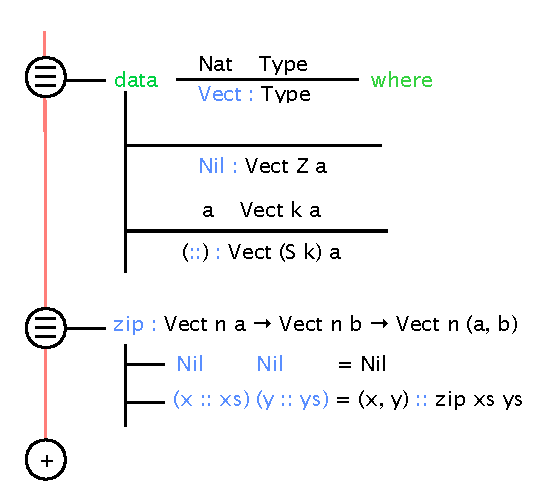
\includegraphics[width=90mm]{diagrams/initial_mockup_design.pdf}
	\caption{Mock-up of a more visual way of representing data types and functions
	in a clear hierarchy.}
\label{fig:initial_mockup_design}
\end{figure}

At the bottom of every construct, there is a round add button, inspired by TouchDevelop, that lets the user add new constructs. These are added to the bottom. 
The round handle buttons connecting each construct to the higher-level vertical line can be used for various code management purposes. 
For example, it is possible to rearrange declarations, clauses, and constructors by dragging these handles. 

Now, if the user wishes to add a new top-level declaration somewhere in the middle of the program, the obvious way would be to use the add button and move the newly created declaration manually. We have, however, designed a faster way.
Reverse-pinching two adjacent handles will create a new declaration between the two existing ones, eliminating the need for rearranging declarations. 
This is a good example of how to use gestures as accelerators for advanced users, and helps us fulfill \textbf{U-4}.
The reverse-pinching gestures is not immediately discoverable (as is the problem with advanced gestures\,\cite[p 141]{nielsen2013mobile}), but power-users will seek faster ways to complete their tasks, for example by reading the accompanying documentation. 
Nielsen and Budiu\,\cite[p 143]{nielsen2013mobile} recommend that you build this sort of redundancy into your app. 
Undo support is implemented as two buttons in the toolbar.
This covers the overall structure of a program in this design. Now we will look at the specifics of declaring functions and data.

% So far: G-3, U-1, U-3, U-4, U-6, F-8, F-9

\section{Function Declarations}
For function declarations we wanted to provide an intuitive flow, using Idris to automate as many steps as possible. 
This meant we had to incorporate initial pattern match creation, case splitting, and automatic metavariable solving into the declaration process.

To be able to declare function types quickly, it was paramount that the interface intelligently presented you with terms that you might have use of.
When a text field takes focus, a context popover with possible terms for that position appears right next to the field. 
The user then only has to move the finger a few centimeters to auto complete the field. 
The usability of this feature depends on how fast and how well the contextual suggestions can be provided.
If the user is looking for a term that is not on the top of the list, it will be necessary to start typing the term manually, until the term list in the context eventually guesses which term is needed. This addresses both \textbf{G-1} and \textbf{G-2}, as well as \textbf{F-7}

% So far: G-1, G-2, G-3, U-1, U-3, U-4, U-6, F-7, F-8, F-9

We did not want to clutter the interface with [+] buttons like Lisping does, so one of the early problems that we needed to solve was to elegantly indicate where new terms could be added.
We came up with the solution seen in Figure \ref{fig:initial_function_editing_design}.
When the user starts typing in the rightmost empty text field, a new text field pops up to indicate that further terms can be added to the type declaration. This is in compliance with \textbf{U-6}.

\begin{figure}
	\centering
		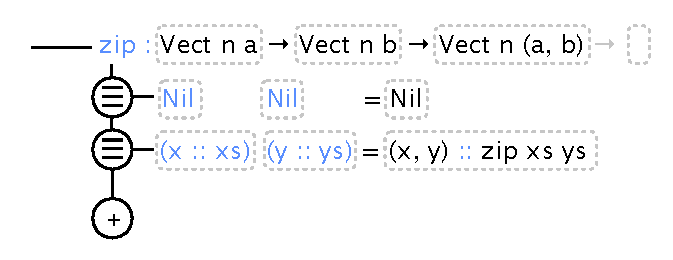
\includegraphics[width=110mm]{diagrams/initial_function_editing_design.pdf}
	\caption{Mock-up of a function in edit mode. Notice the indication that expressions can be
	added at the rightmost end of each line.}
\label{fig:initial_function_editing_design}
\end{figure}

Pressing the plus button on a function with no clauses will add a clause with an initial pattern, with the pattern variables named intelligently. 
Double tapping a pattern variable will perform a case split if possible. 
The use of this gesture is also a non-standard one, and a tip will have to appear one of the first times case splitting is possible.

Finally, metavariables, expressed as three question marks, can be tapped for automatic metavariable solving. 
There should be clear feedback to the user regardless of the outcome of this action.

Together these features leverage the tool support afforded by Idris to fulfill \textbf{F-1}, \textbf{F-2}, \textbf{F-3}, as well as partially fulfilling \textbf{F-5}. To fully fulfill \textbf{F-5}, we must also support deleting functions, as well as cases. This will be addressed in
Section\,\ref{sec:third_design_iteration}. \todo{make sure we describe this}

% So far: G-1, G-2, G-3, U-1, U-3, U-4, U-6, F-1, F-2, F-3, F-7, F-8, F-9

\section{Data Declarations}
Instead of staying visually close to textual Idris, as we had done with function declarations, we decided to try an alternative approach for data declarations, inspired by Epigram.
This resulted in a more visual way of representing data definitions, where a data definition looks less like a function, and more like a logical inference rule.
Any parameters for the type are written as premises, with the type being the conclusion.
Constructors are written in the same manner, with arguments as premises, and the constructed type as the conclusion
Our hope was that this way of declaring data would be more visually appealing, while still enabling a smooth work flow, in accordance with \textbf{U-1}.
The premises of the type constructor and subsequent constructors use the same flow of input as the type declaration of functions.
The reuse of the flow allows the user to learn its behavior once and then use it with a certain feeling of familiarity in the rest of the UI\@.

\begin{figure}
	\centering
		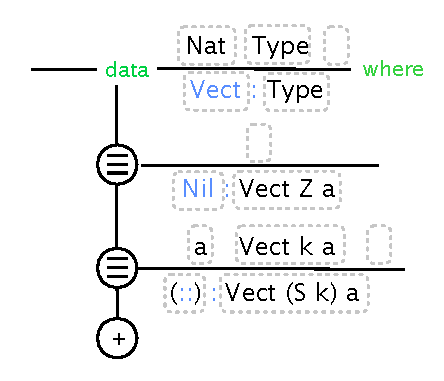
\includegraphics[width=80mm]{diagrams/initial_data_declaration_design.pdf}
	\caption{Mock-up of a data declaration design in edit mode. The syntax
	resembles the 2D Epigram syntax}
\label{fig:initial_data_declaration_design}
\end{figure}

\section{Usability Test}
\label{sec:UsabilityTest}
With a design in hand, it was time to test it. The purpose of this test was to
get an initial idea of how our ideas worked before spending time implementing
them. We created paper cutouts based on our mock-ups to represent the different
elements of the interface, with a test facilitator manipulating the cutouts to
emulate an interactive environment. The procedure of the experiment was inspired by Chapter 10 of ``Observing the user experience'' and a more detailed test report is available in Appendix \todo{Ref}. The report includes a timestamped summary of the test, which we
will sometimes refer to in the following manner: S1.1, which refers to the
first point in the summary for subject \#1.
\todo{reference the book that I referenced in my usability plan (methodology) /N}

\subsection{Participants}
As it is beyond the scope of this project to teach new users about dependent
types, our test participants needed experience with a programming language
featuring dependent types, ideally Idris, prior to our test. This obviously
severely limited the number of readily available candidates. Because we wanted
to conduct later tests with subjects without knowledge of earlier iterations of
the design, we limited ourselves to two test subjects for this first test. An
overview of the test subjects can be see in Table~\ref{table:first_test_subjects}.

\begin{table}[h]
\centering
\begin{tabular}{| l | l | p{5cm} | p{5cm} |}
\hline
Subject & Age & Occupation & Experience \\ \hline
\#1 & 24 & Masters student at IT-University studying programming languages & 6 months experience with Idris, several years of experience with functional languages in general \\ \hline
\#2 & 27 & Masters student at IT-University studying programming languages & 6 months experience with Idris, several years of experience with functional languages in general \\ \hline
\end{tabular}
\caption{Test subjects}
\label{table:first_test_subjects}
\end{table}

\subsection{Session Details}
The test was conducted in a meeting room at the IT University, with three
people present: The test subject, the test facilitator, and a note taker. The
tests were recorded. First, the test subjects were told about the project in
general. They were then told of the overall structure of the test: They would
be given two tasks, with three steps each. Each step would be explained when
they reached it. They were asked to think aloud during the test, and were told to
ask if they felt they had been stuck for a long time. Periodically, we would
ask questions about what they were thinking. At the end of the test, they were asked for general feedback on the test.

\subsection{Tasks}
The two tasks they were asked to complete are listed in Figure~\ref{figure:first_tasks}.
It should be noted that since the test was concerning the interface itself, and
not programming in Idris, the test subjects had access to the definitions for \texttt{Vect} and \texttt{zip} in textual Idris. Refer to Section~\ref{subsec:Idris}
for more on \texttt{Vect} and \texttt{zip}.

\begin{figure}
\centering
\begin{itemize}
	\item \textbf{Task 1}: Define a data declaration for the vector type.
	\begin{itemize}
		\item \textbf{T1.1}: Specify an identifier for the type (\texttt{Vect}), along with its type (\texttt{Nat -> Type -> Type})
		\item \textbf{T1.2}: Specify the Nil constructor (\texttt{Nil: Vect z a})
		\item \textbf{T1.3}: Specify the Cons constructor (\texttt{(::): a -> Vect k a -> Vect (S k) a})
	\end{itemize}
	\item \textbf{Task 2}: Define the zip function for vector type.
	\begin{itemize}
		\item \textbf{T2.1}: Specify the identifier for the function (\texttt{zip}), along with its type (\texttt{Vect k a -> Vect k b -> Vect k (a, b)})
		\item \textbf{T2.2}: Specify the first case (\texttt{zip Nil Nil = Nil})
		\item \textbf{T2.3}: Specify the second case (\texttt{zip x::xs y::s = (x, y) :: zip xs ys})
	\end{itemize}
\end{itemize}
\caption{Tasks for the first usability. The text in parentheses are what we considered the correct answer, and was not given to the test subjects.}
\label{figure:first_tasks}
\end{figure}

\subsection{Issues}
\label{sec:first_issues}
As was expected, several issues were encountered. It was quickly apparent that
the data declarations were the most problematic aspect of the design, and that
we would need to revisit their design. Task 2 on the other hand went quite
smoothly in comparison, and both subjects were impressed by the degree to
which Idris could save them from typing. We have listed the issues we
encountered below. \\ \\
\textbf{I1: Data declarations}.
The main issues our test subjects experienced had to do with the data
declarations. While both subjects had seen this way of writing types
before, it was not immediately clear to them how they should be filled out.
They did eventually get through it, but they required a great deal of help
from the test facilitator. Especially step T1.1 was difficult. (S1.1--8, S2.4, S2.9--15)\\ \\
\textbf{I2: Suggestions for parameterized types}.
When filling in a type, a contextual popover with suggestions would appear. In our mock-up,
these suggestions were always correct. But both subjects wondered how one would
fill in types that take multiple parameters. (S2.29) \\ \\
\textbf{I3: Gesture overload}
One subject wondered how to differentiate gestures for editing versus
gestures for case splitting or autocompletion. For example, double tapping on
text already has an action associated with it. (S2.34) \\ \\
\textbf{I4: Managing contexts}
After having finished step T1.3, both subjects had trouble leaving the editing
context. Only after a great deal of experimentation did they manage to leave
it. Both subjects tried to use the undo and redo buttons to change contexts.
(S1.10--13, S2.21--23)

\subsection{Recommendations}
\label{sec:first_recommendations}
Since issue \textbf{I1} was by far the most problematic issue we discovered, we have
focused on mitigating it in our recommendations. The basic strategy is to make
it easier to understand through examples and help in the interface. If the
changes listed below are not enough, it might be necessary to completely
redesign the data declarations, perhaps by modeling them more closely after how
they look in textual Idris.

\begin{itemize}
	\item \textbf{Re1} (I1): In the text field for inputting the name and type for Data, insert an initial colon (``\texttt{:}''), separating the identifier from the type. This might make it easier to see what goes where.
	\item \textbf{Re2} (I1): Have initial hint text in text input fields, in a light color, which disappears when the fields gain focus. E.g. in the text field for the identifier, it could say ``Identifier'' or ``Name'', while the input field for the type can say ``Type''.
	\item \textbf{Re3} (I1): Differentiate borders around text fields more, to make it clear which fields have been filled, which must be filled, and which might be filled.
	\item \textbf{Re4} (I1): Show the definition for \texttt{Nat} to begin with, so the user can see an example.
	\item \textbf{Re5} (I2): Do not try to fill parameters for types, as we cannot know what they will be. Instead, just leave blank spaces so the user can fill them in.
	\item \textbf{Re6} (I3): To avoid conflict between editing and case splitting/autocompleting, implement a new gesture for ``auto'', perhaps swiping down on a term.
	\item \textbf{Re7} (I4): Implement a button or other UI element that designates the declaration is done. This could be in the form of a check mark, or some other symbol.
\end{itemize}

% So far: G-1, G-2, G-3, U-1, U-3, U-4, U-6, F-1, F-2, F-3, F-7, F-8, F-9

\section{Design Evaluation}
\label{subsec:first_design_evaluation}
While this initial design meets many of the requirements from Section~\ref{sec:GoalsAndRequirements}, there are still issues to resolve.
Specifically, the following requirements are not fully addressed:
\begin{itemize}
	\item \textbf{U-5}: This requires some way to communicate with Idris. The backend required to do this will be covered in Section~\ref{sec:Architecture}, while the design considerations will be covered in
	Section \ref{sec:third_design_iteration}.
	\item \textbf{F-4} and \textbf{F-5}: We have described how to create functions and data declarations, and how one can add and edit clauses and constructors. However, we still need to devise a way to delete these constructs. This will be covered in Section \ref{sec:third_design_iteration}.
	\item \textbf{F-6}: This will be addressed in the next section.
	\item \textbf{F-10}: This will be addressed in Section \ref{sec:third_design_iteration}.
\end{itemize}

Beyond these requirements, the greatest remaining challenge is the data declaration syntax, which we will try to improve in the next design iteration, described in Section~\ref{sec:Implementation}.
We have learned a great deal from this initial design, based on mock-ups and paper cutouts, but for our next iteration, we want to produce a simple prototype app.
Actually implementing our next design will surely uncover many problems not discovered in our mock-ups.
But before we can do this, we need to lay some technical groundwork, which is desicribed in the next section.
%!TEX root = ../Touch Based Idris.tex 
\chapter{Architecture}
\label{sec:Architecture}

We decided to write our app for the Apple iPad, as it is the most prolific
tablet today. We also want to be able to use the various interactive features
available in the Emacs mode for Idris\todo{Ref to requirement}, such as case
splitting and auto completion. One way to achieve this would be to implement
the required functionality directly in our app. But there is a much easier way.
The Emacs mode simply communicates with the Idris interpreter over a socket. 
In this way the Emacs mode can support advanced features that require an
understanding of the underlying semantics of a piece of code, while letting
Idris do all the hard work. We would like to use the same mechanism, but there
are some obstacles. First, we would have to compile Idris for iOS, and make 
sure it works. The Glasgow Haskell Compiler \emph{does} support 
cross-compiling for iOS\todo{Ref}, but the process is not very mature, and
getting Idris (and all of its dependencies) to run on iOS represents an 
unknown amount of work. Second, Apple has very strict rules for interpreting
code on iOS\@. This might make it very difficult to get the app distributed on
the App Store, the only official way to publicly distribute iOS apps.

Because of these factors, we decided to let the Idris interpreter run on a 
host computer, with a thin client running on the iPad, and a server program 
facilitating communication between the client and Idris.

\section{Abstract Syntax}
\label{subsec:AbstractSyntax}
\todo{Give the abstract syntax we've been working with}



\section{Communication}
There are two layers of communication in this setup: one between the client and
the server, and one between the server and Idris. Several different strategies
exist for each layer. 

\subsection{Server -- Idris}
The Emacs mode for Idris communicates to the Idris slave via an s-expression
based protocol\todo{Ref}. This can be avoided by writing the server program in
Haskell, and using Idris as a library instead. This way we can call the
functions we need directly. We still have a problem though, as Idris expects
concrete textual Idris. One solution would involve transforming the AST from 
the client to concrete textual Idris, either on the server or the client. When
receiving replies from Idris, we would then have to parse textual Idris to the
client's AST\@, and send this back. An alternative is to transform the 
client's AST directly to high-level Idris syntax, and bypassing the parsing
steps in Idris, so the functions we need from Idris accept Idris AST directly.
This way we can skip the generation and parsing of concrete Idris. In the end,
we chose this solution, as it seemed cleaner, although it meant learning much
about how Idris is implemented in Haskell.
\todo{Insert diagram showing the two possibilities}

\subsection{Server -- Client}
This layer is somewhat less difficult. The server exposes a simple RESTful API 
over HTTP\@. This makes it easy for the client and server to communicate across
different networks. When transferring a program from client to server, we
serialize the client AST to JSON\@.

\section{Server}
The architecture of the server is very simple, and consists of two main 
layers. The outer layers uses the Snap Framework\todo{Ref} to implement the 
web-services. This layer also handles marshaling to and from JSON\@, which is 
implemented using the Aeson library\todo{ref}. The inner layer handles the 
transformations to and from the Idris high level syntax, and performs the 
actual operations, such as case splitting.

\todo{Insert diagram showing overall architecture}

\section{Client}
The iPad client is, of course, written in Objective-C as is the standard. The
software architecture is based on the Model View ViewModel (MVVM) design 
pattern\todo{ref}, which is an extension of the popular Model View Controller 
(MVC) pattern. MVVM nicely separates business logic from the view-related
display logic, and the latter is stored in the ViewModel object to unclutter 
the controller object, which in turn only contains business logic.

The model hierarchy resembles the abstract syntax from Section \ref{subsec:AbstractSyntax},
where the type constructors are represented as abstract classes on the client
and the specific constructors, concrete classes. Note that abstract classes in
Objective-C are only abstract by convention, as the language does not directly
support this feature.

To handle asynchronous network calls as well as input from the user we have
used the ReactiveCocoa (RAC) Framework\todo{ref}, which is an Objective-C framework for
Functional Reactive Programming\todo{ref}. In RAC almost everything is a
signal. Signals follow the Future/Promise design pattern and provide an
efficient way of handling future events.

\todo{The following needs to be integrated somehow}

This prototype consists of a lot of custom elements, and the way that they work
together has been challenging to implement. Figure~\ref{fig:clientViewArchitecture} shows a simplified class diagram of the
client. It shows the UI classes of the project to give an idea of
the resemblance to the abstract syntax. As with the abstract syntax there are
two ``levels'' of views --- top level and input level. The MainView holds a
number of top level declarations, that each hold a number of input views. The
InferenceRuleView is used by the DataDeclarationView only.

A GroupInputView contains one or more AbstractInputViews. This way of building
the interface makes it easy to wire input views to the underlying model object
hierarchy, as it is the same type of nesting we have with terms. \todo{Explain
what the group input view is and how it can be customized}

\begin{figure}
	\centering
		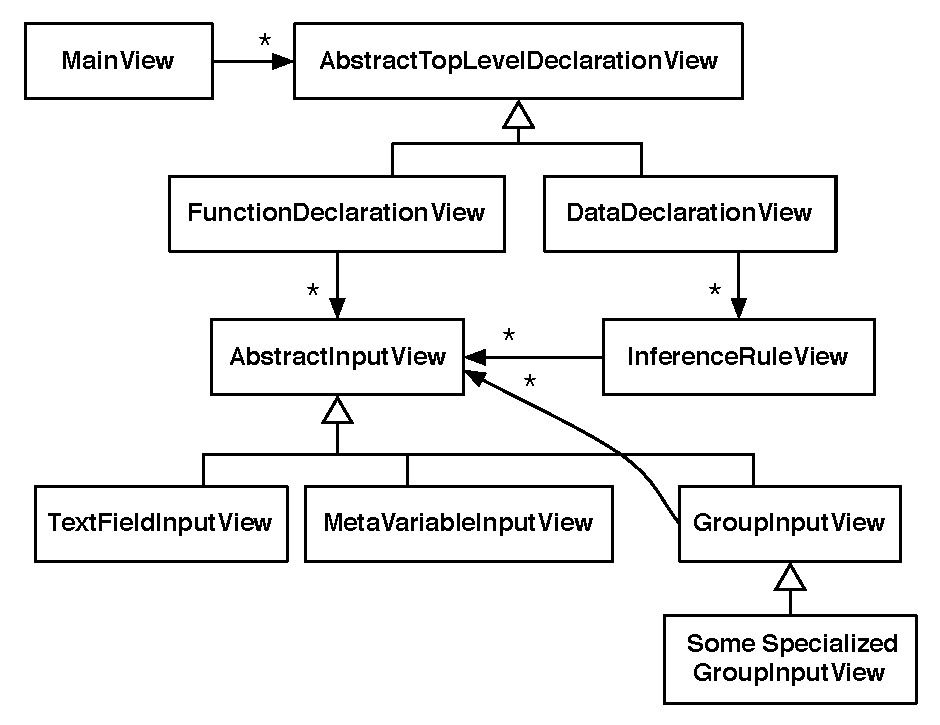
\includegraphics[width=110mm]{diagrams/client_side_class_diagram.pdf}
	\caption{A subset of the client-side diagram showing how the view hierarchy
	almost mirrors the Abstract Syntax tree.}
\label{fig:clientViewArchitecture}
\end{figure}












%!TEX root = ../Touch Based Idris.tex
\chapter{Second Design Iteration}
\label{sec:Implementation}

With an architecture in hand, it was time for the next design iteration.
As we mentioned in Section~\ref{subsec:first_design_evaluation}, several requirements and issues were still to resolved, and we felt the biggest remaining issue was the data declaration syntax.
It was the goal to create a prototype running on the iPad, ready for usability testing with a larger group of participants than in the mock-up phase.
Unfortunately, technical issues arose when implementing the many custom UI elements for the iPad prototype, which meant we had to be significantly less ambitious with regards to design changes from the first iteration.

\section{Data Declarations}
\label{subsec:second_data_declarations}
Our first priority was to improve the data declarations from our initial design. 
We followed \textbf{Re1} by splitting the name for the data and its type into two text fields, with a colon separating them. 
We also followed \textbf{Re2} by including text hints as to what should be in a text field.
These hints disappear as soon as the field gains focus.
The outlines around input fields were also changed to differentiate between fields that had been filled out, and fields that were yet to be filled out, as stated in \textbf{Re3}.
All these changes can be seen in Figure~\ref{fig:data_declaration}.

\begin{figure}
	\centering
		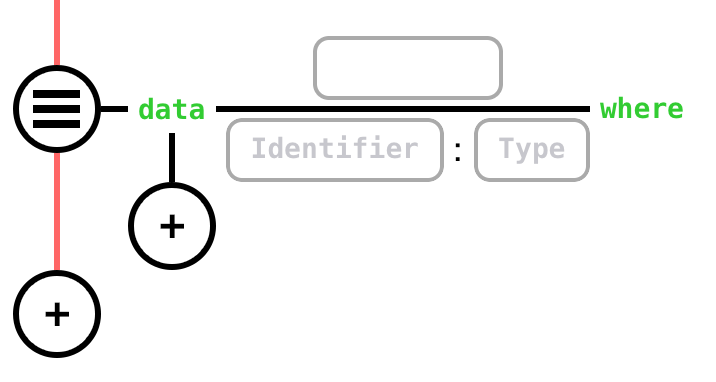
\includegraphics[width=70mm]{diagrams/data_declaration.png}
	\caption{A data declaration before the user has filled out anything.}
\label{fig:data_declaration}
\end{figure}

\section{Other Changes}
\label{subsec:other_changes}
Due to delays caused by the technical issues mentioned above, very few other changes, besides small tweaks, made it into this iteration.
In fact, one feature that was present in the original design did not make it into the prototype app, the TouchDevelop-like focus shifting, where different top-level elements would be in focus at different times. In this prototype all elements are in focus all the time. This goes against \textbf{U-6} and \textbf{F-9}. 
The final design can be seen in Figure~\ref{fig:initialiPadInterface}.

\begin{figure}
	\centering
		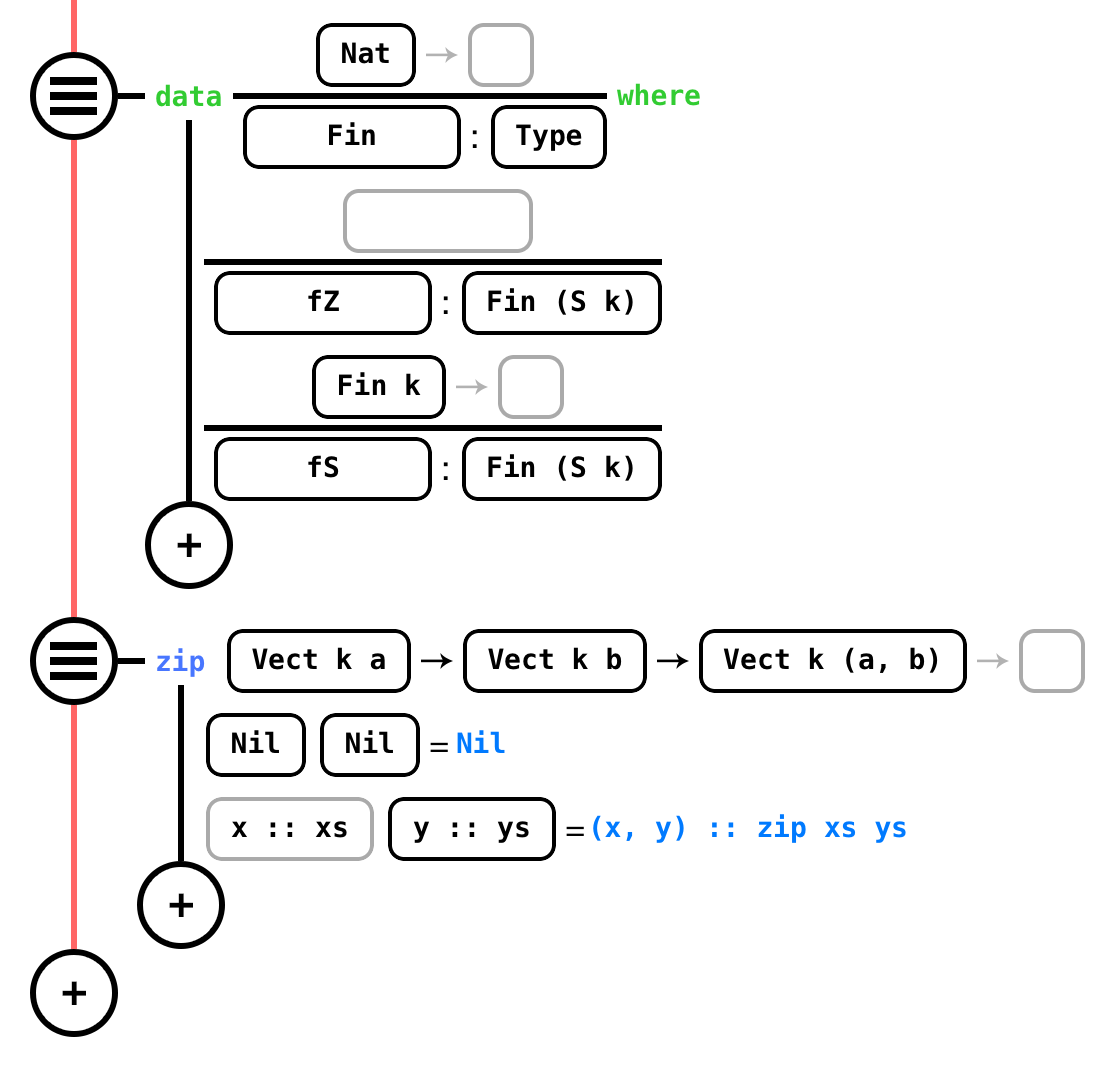
\includegraphics[width=110mm]{diagrams/ipad_interface.PNG}
	\caption{The initial iPad interface.}
\label{fig:initialiPadInterface}
\end{figure}

\section{Second Usability Iteration}
\label{sec:SecondUsabilityTest}
The greatest change in the second usability test was the fact that it was
performed on an actual iPad, using a prototype interface. The full report is
included in Appendix \todo{insert ref}. As in the first test, S2.4 refers to
the fourth point in the test summary for subject 2.

\subsection{Participants}
For our second usability test, we used two subjects from the first test,
subject \#1 and \#2. Their input was interesting, as they already had some
experience with the ideas in our representation from the mock-up test.
Hopefully this would let them focus more on the interactions with interface,
and less on learning a new way of presenting data. Subjects \#3 and \#4 had
never seen the interface before, and as such represented totally new users.
Their feedback was also very useful, as this iteration tried to make the first
time experience less frustrating.

\begin{table}[h]
\centering
\begin{tabular}{| l | l | p{5cm} | p{5cm} |}
\hline
Subject & Age & Occupation & Experience \\ \hline
\#1 & 24 & Masters student at IT-University studying programming languages & 7 months experience with Idris, several years of experience with functional languages in general \\ \hline
\#2 & 27 & Masters student at IT-University studying programming languages & 7 months experience with Idris, several years of experience with functional languages in general \\ \hline
\#3 & 27 & Masters student at IT-University studying programming languages & Very little experience with Idris. 1 year experience with Coq. Several years of experience with functional languages in general \\ \hline
\#4 & 23 & Masters student at IT-University studying programming languages & 6 months experience with Idris. Several years of experience with functional languages in general \\ \hline
\end{tabular}
\caption{Test subjects}
\label{table:second_test_subjects}
\end{table}

\subsection{Session Details}
Like the first test, this test was conducted in a meeting room at the IT
University, with three people present: The test subject, the test facilitator,
and a note taker. The tests were recorded. This time the test consisted of four
tasks, with the first task designed to get the subjects acquainted with the
data declarations, as per \textbf{Re4}. The next two tasks were identical to the first test, the
definition of the \texttt{Vect} data type and the \texttt{zip} function for
\texttt{Vect}. The final task concerned the manipulation of order of
declarations in the program they defined. As the app was still at prototype
stage, several bugs occurred during the subjects' use of the app. In these
cases the nature of the bug was quickly explained, and the facilitator
explained how to work around the issue.

\subsection{Tasks}
The four tasks they were asked to complete are listed in 
Figure~\ref{figure:second_tasks}.
As in the first test, the test subjects had access to the definitions for
\texttt{Vect} and \texttt{zip} textual Idris. See Section~\ref{subsec:Idris}
for more on \texttt{Vect} and \texttt{zip}.

\begin{figure}
\centering
\begin{itemize}
	\item \textbf{Task 1}: The user is shown the \texttt{Nat} and \texttt{Fin} data declaration in the program.
	\begin{itemize}
		\item \textbf{T1.1}: Describe the \texttt{Nat} type.
		\item \textbf{T2.2}: Describe the \texttt{Fin} type.
	\end{itemize}
	\item \textbf{Task 2}: Define a data declaration for the vector type.
	\begin{itemize}
		\item \textbf{T2.1}: Specify an identifier for the type (\texttt{Vect}), along with its type (\texttt{Nat -> Type -> Type})
		\item \textbf{T2.2}: Specify the Nil constructor (\texttt{Nil: Vect z a})
		\item \textbf{T2.3}: Specify the Cons constructor (\texttt{(::): a -> Vect k a -> Vect (S k) a})
	\end{itemize}
	\item \textbf{Task 3}: Define the zip function for vector type.
	\begin{itemize}
		\item \textbf{T3.1}: Specify the identifier for the function (\texttt{zip}), along with its type (\texttt{Vect k a -> Vect k b -> Vect k (a, b)})
		\item \textbf{T3.2}: Specify the first case (\texttt{zip Nil Nil = Nil})
		\item \textbf{T3.3}: Specify the second case (\texttt{zip x::xs y::s = (x, y) :: zip xs ys})
	\end{itemize}
	\item \textbf{Task 4}
	\begin{itemize}
		\item \textbf{T4.1}: Move the \texttt{Vect} declaration up below \texttt{Nat}.
	\end{itemize}
\end{itemize}
\caption{Tasks for the second usability test. The text in parentheses are what we considered the correct answer, and was not given to the test subjects.}
\label{figure:second_tasks}
\end{figure}

\subsection{Issues}
\label{sec:second_issues}
We discovered many new issues in this usability test, which is not
surprising. In the first test, the facilitator took over the iPad's role, by
manipulating the mockups. This masked many flow and ease of use issues, which
have now been identified. During the test, several bugs were encountered. These
are not listed below, as they are not inherent to the design, but rather
results of the prototypical nature of the app.
\\ \\
\textbf{I5: Too many input fields}.
Most of the users reported that all the grey, unfilled input fields were
confusing. 
This will hopefully be partially solved by the focusing system. (S1.20, S2.2, S3.29b)
\todo{Insert screenshot}
\\ \\
\textbf{I6: Writing data declaration}
Everyone was able to decipher the data declarations almost immediately, but
all but one had trouble writing the \texttt{Vect} data declaration. Especially
the distinction between the premise area and the conclusion area seemed
problematic. (S1.1--1, S3.11--18, S4.3--7)
\\ \\
\textbf{I7: Arrows in data confusing}
The use of arrows in the premise area is confusing, as it implies a function. 
(S4.4)
\\ \\
\textbf{I8: Suggestions for parameterized types}
This issue persists from the original design. The subjects found it irritating
that after choosing a suggestion, they would have to manually change the
parameters using the standard iOS text editing facilities. Multiple subjects
mentioned that it broke their flow. (S1.10, S2.7, S3.15)
\\ \\
\textbf{I9: Lack of auto-closing parentheses and quotation marks}
We observed that users spent too much time navigating the virtual keyboards to
close pairs of symbols, when this can be done automatically.
\\ \\
\textbf{I10: Common symbols inaccessible}
In a similar vein, we noticed that some symbols commonly used when programming,
e.g. ``<'', took too long to find in the virtual keyboard.
\\ \\
\textbf{I11: Poor flow between input fields}
To move from one input field to the next, the subjects must manually tap each
input field. This broke the subjects flow. (S1.21, S3.30c)
\\ \\
\textbf{I12: Program can look cluttered}
After finishing all the tasks, the subject's program started to look cluttered.
This should also be alleviated by the focus system.
\todo{Insert screenshot} (S3.29a)
\\ \\
\textbf{I13: Few definitions visible}
Related to Issue I12, definitions are quite large, so only a few are visible at
any time. This can make it hard for the subject to get an overview of their
work.
\\ \\
\textbf{I14: Unclear how to specify implicits and identifiers for arguments}
Some parts of the syntax have not been determined. Some of the subjects
wondered how one would make an argument implicit. (S1.9, S4.13)

\subsection{Recommendations}
\label{sec:second_recommendations}
As we did not have time to implement all the recommendations from our first iteration, they still apply to this iteration, even though they are not listed again here.
Some issues (such as I5) are partially due to the fact the prototype was missing certain features, such as the focus system.
We have not added recommendations for these issues if we believe the not yet implemented features will improve them.

\begin{itemize}
    \item \textbf{Re8} (I5): When centering text that includes an extra input field, center the text without the input field. \todo{Insert screenshot}
    \item \textbf{Re9} (I7): Use semicolons instead of arrows in the premise area of data declarations.
    \item \textbf{Re10} (I8): When showing types that take parameters, indicate these parameters in the popup. Then, after choosing one, create two new sub input fields, with their own suggestions. Make sure there is a good flow between these fields.
    \item \textbf{Re11} (I9): Automatically close pairs of symbols.
    \item \textbf{Re12} (I10): Include a shortcut bar for symbols.
    \item \textbf{Re13} (I11): After filling a field, automatically move input to next field. Perhaps include a button to move back and forth between fields.
    \item \textbf{Re14} (I12): Include more spacing between fields.
    \item \textbf{Re15} (I13): Include a cheat sheet of some kind, showing constructors and types for functions.
    \item \textbf{Re16}: In general, it might be good to separate text editing from general manipulation of the program. Text editing could occur in popups or a dedicated text input field, freeing gestures for other uses when manipulating the structure of the program.
\end{itemize}

\section{Design Evaluation}
\label{second_design_evaluation}
Unfortunately there were several recommendations from the first iteration that did not make it into this design. 
The missing functionality mentioned in Section~\ref{subsec:first_design_evaluation} also did not make it into this version.
While it is regrettable that we did not have a chance to test our recommendations or new features, the mere fact that we tested our design on an iPad led to a wealth of new insight.
We discovered many issues with the existing design that were only apparent when the design was put to use on a device. 
The final unmet usability requirement, to do with error handling (\textbf{U-6}), along with the functional requirements concerned with editing declarations (\textbf{F-4}, \textbf{F-5}) and quickly accessing special characters (\textbf{F-10}) will be addressed in the final design, presented in Section~\todo{ref}. 
This final design will also explore the recommendations from the first iteration (see Section~\ref{sec:first_recommendations}) that were not explored here, and experiment with a new way of declaring data.

%!TEX root = ../Touch Based Idris.tex
\section{Third Design Iteration}
In this, the third and final, iteration of our design, we present some major changes to how data declarations are represented.
We also reevaluate the way text input is handled, as the previous iterations were mainly concerned with how declarations are created, and not with how they are changed or removed.
Unlike the two prior iterations of the design, this version has not been through a usability test, although a plan for one is included in Section~\ref{third_usability_test}.

\subsection{New Input model}
% Re5/10, Re6, Re15, Re16
\label{subsec:new_input_model}
As the two first design iterations did not go into much detail on how text input was handled, we discovered several issues regarding text input, especially when editing existing text.
Because of these issues, we decided to reevaluate how input is handled.

The text fields of the first and second design are not structured at all, they are simply plain text fields, using the standard text input gestures and customs.
This gave rise to overloading of gestures, as was also the case in the Lisping editor (see Section~\ref{subsub:Lisping}).
For example, if the user wants to case split a pattern variable, the user must double tap it, but that gesture is already in use by the text field, as seen in \textbf{I3}.
Besides these overloading issues, working with plain text on a touch interface is problematic in general, and it is hard to avoid using the virtual keyboard for many operations.

One possible solution would be a more structured approach to text input, as in EastWest (see Section~\ref{subsub:Eastwest}).
This would let us separate text input from the manipulation of programs, as per \textbf{Re16}, negating \textbf{Re6}.
This could be implemented by limiting all text entry to what we call the context popover, shown in Figure~\ref{fig:new_design_popover}.
The context popover was inspired by \textbf{Re5} and \textbf{Re10}, and also fulfills \textbf{Re15} by providing the user with an overview of what is available.

\begin{figure}
	\centering
		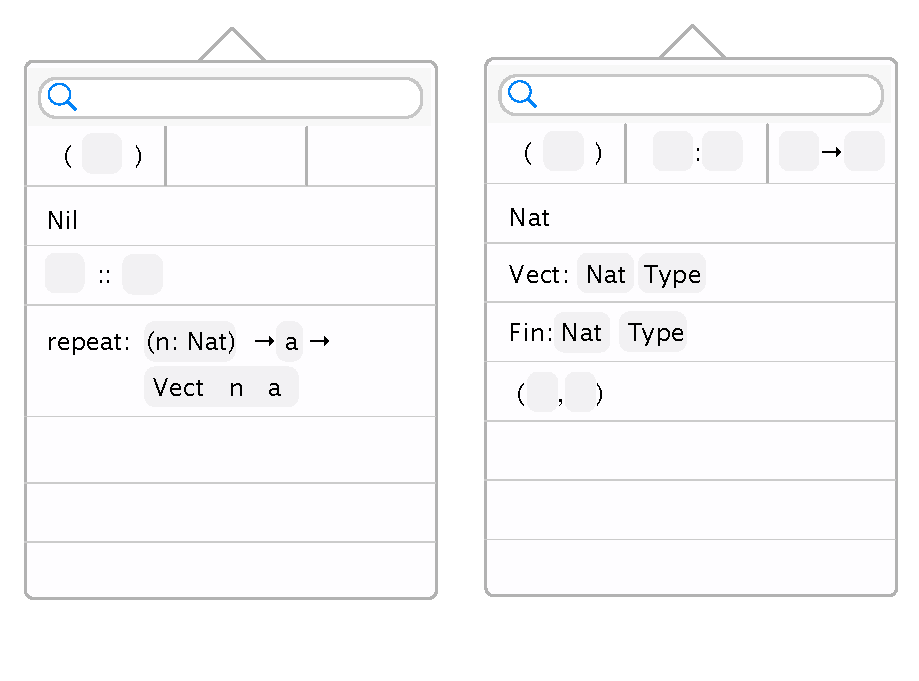
\includegraphics[width=110mm]{diagrams/final_design_popover.pdf}
	\caption{The context popover. Left: How it looks when a \texttt{Vect} is
	expected. Right: How it looks when defining a new type constructor.}
\label{fig:new_design_popover}
\end{figure}

In this design, writing a program would consist of filing a series of holes for terms by choosing applicable functions and constructors from the popover, and only using the virtual keyboard for writing constants, variable names, or searching.
Once a term has been filled, it can be dragged around, and gestures can be used to manipulate it without clashing with text input gestures.
To edit a term, the user can double tap it to bring up the context popover, with any new choices replacing the old choice.
This design means there would be no risk of the user making syntax errors, but on the other hand there would be less freedom to approach the programming task in the way the user prefers, which will be addresed in Section~\todo{Ref}.

The content of the context popover can be sorted by both the frequency of use of a specific item, as well as locality, such that functions defined in the same file are given precedence over library functions.
Getting this heuristic right would require testing with users.

Populating the context popover would require a feature not currently available in the Idris slave mode: searching by type.
For the popover to work, we would have to be able to ask Idris for all constructors and functions that have some specific type, for example \texttt{Nat -> String}.
We believe this to be a feasible extension to Idris. 

\subsection{Managing Program Structure}
% F4, F5, Re7, Re13, Re14
Figure~\ref{fig:new_data_declaration} shows two top-level declarations
where none of them are in focus. 
In this state the programmer can get a clear overview of the program without any clutter. 
Tapping anywhere on a declaration takes the user to the state seen in Figure~\ref{fig:new_design_data_in_focus}, where the elements of the declaration are bigger and easier to tap.
The check mark button removes focus from the current declaration and should help mitigate \textbf{I4} by giving the user a clear way to indicate that he is done with editing, following \textbf{Re7}.
Tapping other top-level declarations will switch the current editable declaration to non-editable and switch the tapped top-level declaration to editable.

\begin{figure}
	\centering
		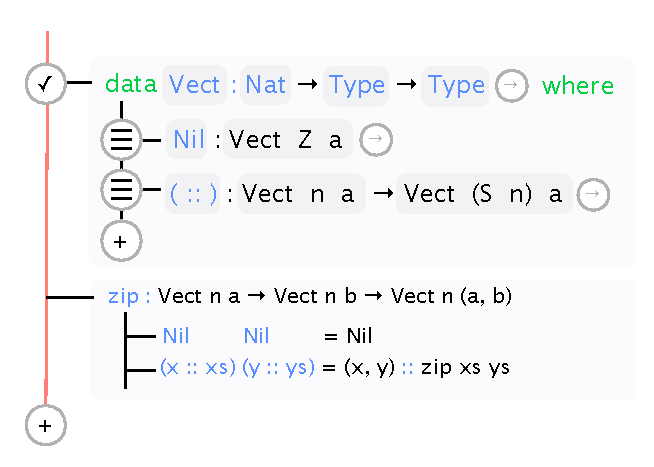
\includegraphics[width=100mm]{diagrams/final_design_top_dec_in_focus.pdf}
	\caption{The new design with a data declarations in focus. The code becomes
	bigger and easier to tap}
\label{fig:new_design_data_in_focus}
\end{figure}

\begin{figure}
	\centering
		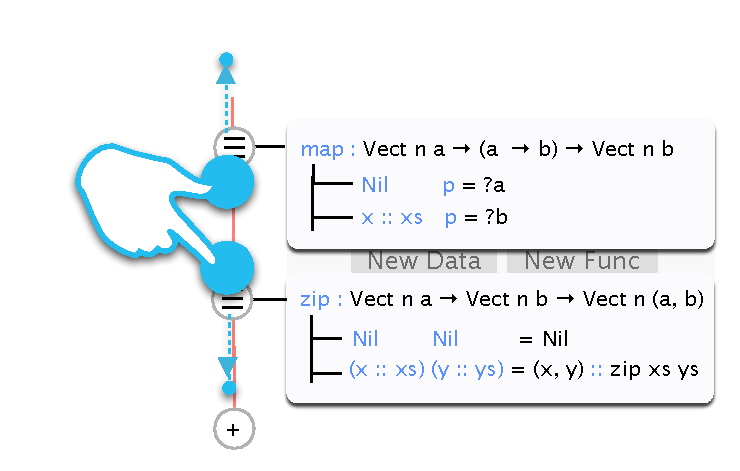
\includegraphics[width=110mm]{diagrams/new_function_reverse_pinch.pdf}
	\caption{When reverse pinching two adjacent handles for top-level
	declarations, a new top-level declaration appears between the old ones.}
\label{fig:new_function_reverse_pinch}
\end{figure}

We have decided to keep our original design for creating new top-level
declarations. Either, the programmer can use the [+] button at the bottom of
the program, or he can reverse-pinch two adjacent top-level declarations to
create a new one between them. This also works for creating constructors
between existing constructors in data declarations.

Now that the representation of a term is no longer overloaded with conflicting
gestures, we can incorporate drag-to-rearrange. Figure\ref{fig:design_drag_to_garbage}
shows an example of this behavior. When the user begins to drag a term, it pops
out of its current position, and can be rearranged with other terms on the same
line. Also, while the user is dragging the term, a trash icon appears in the
upper right corner of the screen, to indicate that it can be deleted. Experienced users can flick the term towards the trash icon, whereas novice users will just drag it.
Clauses in functions and constructors for data can also be deleted in this way, thus fulfilling \textbf{F-4} and \textbf{F-5}.

\begin{figure}
	\centering
		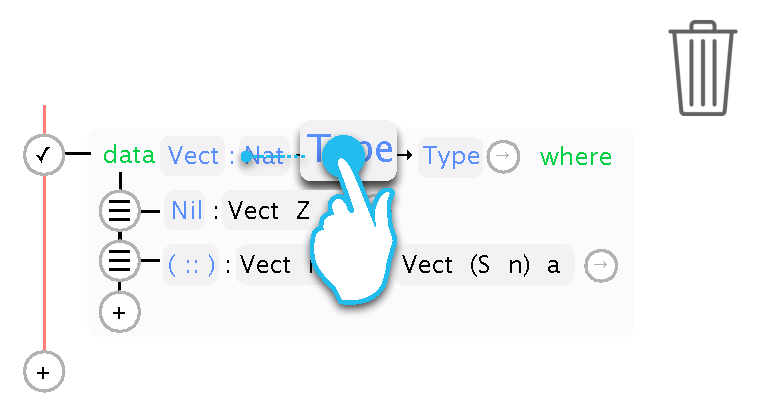
\includegraphics[width=110mm]{diagrams/design_drag_to_garbage.pdf}
	\caption{When reverse pinching two adjacent handles for top-level
	declarations, a new top-level declaration appears between the old ones.}
\label{fig:design_drag_to_garbage}
\end{figure}

\subsection{Data Declarations}
\label{subsec:new_design_data_dec}
Due to the many issues uncovered concerning the Epigram-inspired data declarations (described in \textbf{I1}, \textbf{I6} in Section~\ref{sec:first_issues} and Section~\ref{sec:second_issues}, respectively), and our failure to improve the situation substantially, we decided to try a more traditional approach to data declarations.

\begin{figure}
	\centering
		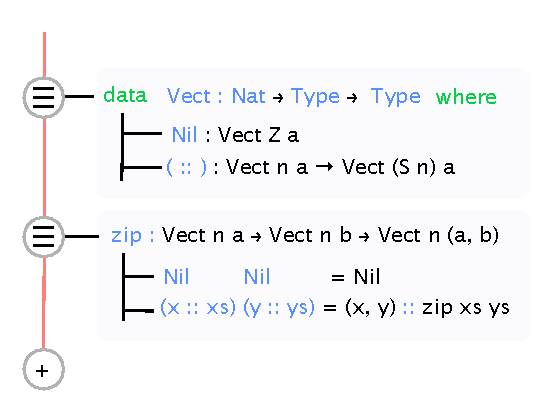
\includegraphics[width=100mm]{diagrams/final_design_nothing_in_focus.pdf}
	\caption{The new data declaration, along with the familiar function declaration.}
\label{fig:new_data_declaration}
\end{figure}

The new data declaration is shown in Figure~\ref{fig:new_data_declaration}.
It is very reminiscent of how data is declared in textual Idris, and in other functional programming languages.
It is our hope that this design will make it easier to read and write data declarations for users not familiar with the interface. This change obviates \textbf{Re8} and \textbf{Re9}, and potentially solves \textbf{I1} and \textbf{I6}.

\subsection{Function Declarations}
\label{subsec:new_design_function_dec}
The function declarations work much the same way as the data declarations
except for the extra support for initial pattern match creation, case splitting
and meta variable solving.

The initial pattern match creation is still done by pressing the [+] button to
add a new clause. Case splitting can no longer be done by double tapping a
term, as this would toggle it to edit mode. Instead, the user drags the term
down and a new clause appears like it can be seen in Figure~\ref{fig:case_splitting}.

\begin{figure}
	\centering
		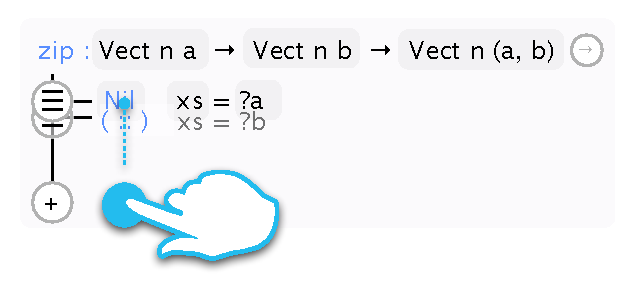
\includegraphics[width=100mm]{diagrams/design_case_splitting.pdf}
	\caption{Case splitting is done by dragging a term down until a new clause
	appears.}
\label{fig:case_splitting}
\end{figure}

Meta variable solving is managed in an even simpler way. If a term starts with
a question mark like in Figure~\ref{fig:case_splitting} then a single tap will
tell the compiler to try and automatically solve the meta variable. Double
tapping it will as always make the term toggle to edit mode.

\subsection{Virtual Keyboard}
%F-10
\label{subsec:virtual_keyboard}
We have also extended the virtual keyboard with a shortcut bar, inspired by the one in Textastic, as can be seen in Figure~\ref{fig:design_keyboard}.
Each button in the bar can hold several symbols.
To select a specific symbol, the user first touches the button, then swipes in the direction of the desired symbol, and lets go.
For example, to select the plus symbol, the user would touch the leftmost button in the bar, then swipe left.
The bar also features a button to the far right that lets the user add a new argument when specifying types. 
This design solves requirement \textbf{F-10}. 

\begin{figure}
	\centering
		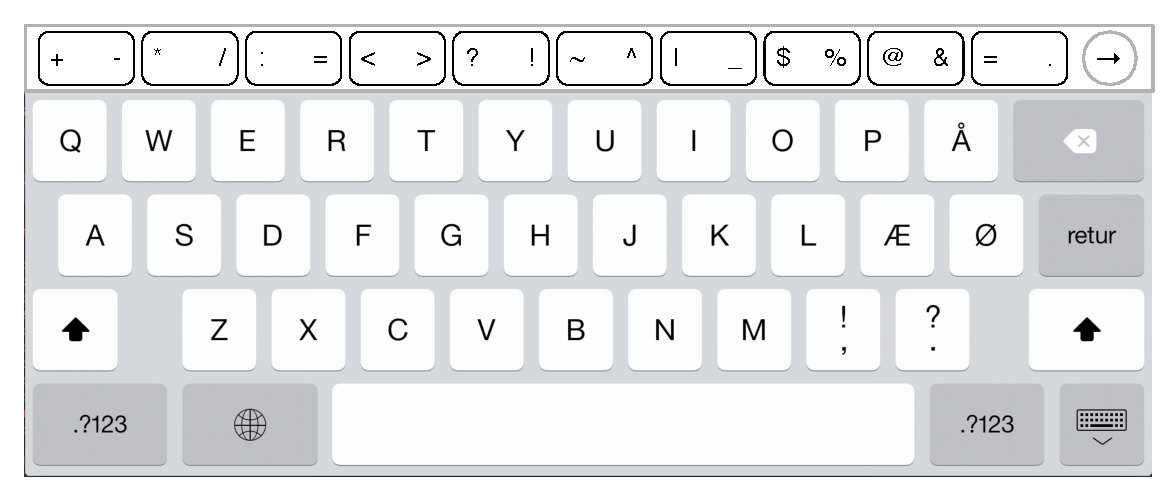
\includegraphics[width=115mm]{diagrams/design_keyboard.pdf}
	\caption{The Textastic-inspired keyboard with common symbols.}
\label{fig:design_keyboard}
\end{figure}

\subsection{Error Handling}
% U-6
\label{subsec:error_handling}
So far our usability tests have not focused on error handling at all, but in this iteration it is time to begin focusing on this important part of the edit-compile-test cycle.
We propose that errors are indicated by a red background on the term that contains an error. 
Tapping on this term will bring up the context popover that will indicate the error.
For example, say the user has written the term \texttt{foo (bar a b) 2}.
Somewhere else, \texttt{foo} is redefined so the second argument is no longer needed.
In this case, the \texttt{2} would be highlighted in red, and the user can then flick it to the trash, as described above.
This feature solves \textbf{U-6}.

\subsection{Third Usability Iteration}
\todo{Rename all usability sections to "Number Usability Test"}
\label{subsec:third_usability_test}
With this new design we feel that the user interface has reached a maturity
level where it is important to focus on the server-side for a while. In the
next usability test, the solution's edit-compile-test cycle should be tested to
a larger extent, and that requires a working back-end. The following usability
test cases assume that we have a working prototype with the new design
implemented as well as a working server that can serve compilation results.

The participants of the usability test should again be a mix of programmers
that are new to the platform and some that are not. Other than that, they
should be screened in the same way as in our second usability test (Section
\ref{sec:SecondUsabilityTest}).

What we specifically wish to test in this next usability test is:

\begin{enumerate}
	\item The flow when declaring new data types and functions. This includes the auto-completion feature and the context popover
	\item The understandability of the way we now declare data types
	\item The focus system, where only one top-level declaration is in focus at a
	time. Can users maneuver in and out of declarations in a fairly easy way?
	\item Editing right-hand sides that have already been added.
	\item Deleting terms by flicking them and rearranging them by dragging.
	\item Deleting top-level declarations, clauses, and constructors
\end{enumerate}

It does not make sense to draw up an exact usability test plan like the ones we have made in previous usability
at this point. We would need to have a working version of the solution before a precise test plan can be made. Also, the few points listed above could easily amount to more than 10 tasks, which is more than can be completed in an hour with a participant. For this reason we would have to prioritize the focus of the test, and that can only be done when we have the new solution in our hands and decide what features we are most confident about. 

%!TEX root = ../Touch Based Idris.tex
\chapter{Evaluation}
\label{sec:Evaluation}
In this section we will evaluate our final design against the goals and requirements listed in Section~\ref{sec:GoalsAndRequirements}.
Fulfilling the functional requirements and usability requirements is a
prerequisite to fulfilling our goals, so we will evaluate those first.

\section{Requirements}
\begin{itemize}

\item \textbf{U-1}: Program structure is clearly communicated trough the data and function declarations described in Section~\ref{sec:third_design_iteration}.
Only one of four test participants of the second usability iteration had minor
issues figuring out the program structure (Appendix \ref{chap:SecondUsabilityTest},
S1.1-3, S2.1-3, S3.1-7, S4.1-2).
\item \textbf{U-2}: We use few, non overlapping touch gestures to accomplish specific goals,
but it should be usability tested as described in Section \ref{subsec:third_usability_test}.
We are confident that our combination of touch gestures will work better than
what we achieved in the initial iPad prototype.
\item \textbf{U-3}: By explicitly giving focus to one top-level declaration at
a time we can ensure that the visual representation of the program scales just
as well as a purely textual program would. Top-level declarations not in focus
will not take up more screen real-estate than in a free-text editor. This
behavior is described in Section \ref{subsec:managing_program_structure} and
should be usability tested in the third usability iteration.
\item \textbf{U-4}: We include several accelerators, such as reverse-pinch to create new declarations, that do not impede the novice user, and thus meet this requirement.
Another feature worth mentioning is the auto completion feature of the editor,
which should speed up the user's programming speed considerable making for a
faster edit-compile-test cycle.
\item \textbf{U-5}: Syntactical errors are prevented through the use of structured editing, and semantic errors are handled in a simple way, showing the user where the error is directly in the program.
This was described in Section\,\ref{subsec:error_handling}.
\item \textbf{U-6}: By only showing input areas when the current declaration is being edited, we keep clutter to a minimum, while still making it clear where the user can make changes.
\todo{reference difference between Lisping figure, iPad prototype figure with a
lot of grayed out holes, and the new design that does better than both of these}
\item \textbf{F-1}, \textbf{F-2}, \textbf{F-3}: Initial pattern matching, case splitting of pattern variables, and automatic metavariable solving is supported, and described in Section~\ref{subsec:new_design_function_dec}.
\item \textbf{F-4}, \textbf{F-5}: The user can add, delete, and edit data declarations, as described in Section~\ref{subsec:managing_program_structure} and Section~\ref{subsec:new_design_data_dec}
and function declarations, as described in Section~\ref{subsec:managing_program_structure} and Section~\ref{subsec:new_design_function_dec}.
\item \textbf{F-6}: By letting the Idris compiler run on a host computer (see Section~\ref{sec:Architecture}), we believe we do not break any App Store guidelines. However, in the end this is up to the App Store review team, and we cannot know without actually submitting an app.
\item \textbf{F-7}: The user can get an overview of what is available through the context popover, described in Section~\ref{subsec:new_input_model}
and depicted in Figure \ref{fig:new_design_popover}.
\item \textbf{F-8}: Undo support is provided by buttons in the interface, which we believe improves the undo-experience considerably
compared to shaking the device.\todo{Double check that we describe this in our
design}
\item \textbf{F-9}: This requirement is met through the focus system described in Section
\ref{subsec:managing_program_structure}.
\item \textbf{F-10}: This requirement is met by the context-dependent virtual keyboard described in Section~\ref{subsec:virtual_keyboard}.

\end{itemize}

\section{Goals}
Our goal was to design an editor that leverages Idris to provide a usable solution for touch based editing, which delivers a competitive edit-compile-test cycle, with minimal use of the virtual keyboard, while remaining eligible for the Apple App Store.
We believe our latest design will make the fulfillment of these goals possible. 
Since the latest design was not tested with users, we can only guess at how effective
it would be at fulfilling G-2 and G-3. The edit-compile-test cycle has potential to be a lot faster than existing solutions due to the minimal reliance
on the virtual keyboard and the heavy reliance on auto completion. On the other
hand we have not yet tested this flow due to technical reasons, and we do have
a longer compiler response time, as the compiler runs on a remote server
instead of locally on the device. It is our hope that the advanced auto
completion feature will make up for the limitations of the distributed
architecture. This architecture was necessary to fulfill G-4.

We are convinced that with further iterations and more usability tests, our design could result in a product that is better suited for touch-based programming than existing
solutions. \todo{maybe mention that it will take many hours to complete this
project and to get those results}

%!TEX root = ../Touch Based Idris.tex
\chapter{Reflection}
\label{sec:Reflection}
In this chapter, we will reflect on some of the challenges we faced, as well as on the choices we made.

\section{The Third Design Iteration}
In the third design iteration (see Chapter~\ref{sec:third_design_iteration}), we proposed large changes to the design.
In itself this is not a problem, but these changes came at a point where we no longer had time to test them.
We always planned to propose a last design after our final tests, with the goal of trying to cover any issues we discovered, however we had not planned to propose such radical changes, featuring many unknowns.
We could have proposed less drastic changes, but these would have left many issues unaddressed.

The biggest unknown is probably how the more structured approach would work out in practice.
Structured editors are not nearly as common as plain text editors, but we have not had the opportunity to look into why this is. 
One can imagine that one reason might be an increased learning curve. 
Another might be the more restricted workflow they present.
If this project was continued, these questions would need to be explored. 

\section{Process}
The initial project plan had a lot of focus on prototype development, but we
soon realized that we had to shift focus towards usability testing. We
originally intended only to provide a plan for usability testing and not
actually carry it out, but we quickly discovered that designing a usable prototype was more or less impossible without
participation from the intended users. We could probably have carried out one more
usability iteration if we had not focused on the server-side at all, and that
would most likely have resulted in a better user interface. With our
current approach we are closer to being able to fully test the
edit-compile-test cycle than we would have been only focusing on usability.

In almost all previous projects we have spent too little time on the initial literature
study, so in this project we wanted to focus more on it as is reflected by the
length of Chapter~\ref{sec:Analysis}. Retrospectively, we could have used some of this time to further develop our design and prototype. 

\section{Constraining Factors}
During this project we have encountered an incredibly high amount of unforeseen constraining factors. Some of the simplest things turned out to require demanding workarounds due to the strict rules of the iOS platform and the large number of technologies and languages that had to work in combination in the finished product.

A good example of the unforeseen complexity of the simplest of components was writing a JSON parser on the client side. Most often this is a tedious task that can be left to standard or third party libraries, which was also the case on the server side in Haskell. A data definition with $n$ constructors in Haskell corresponds to one abstract class with $n$ concrete classes inheriting from the abstract class in Objective-C. It turns out that none of the most popular Objective-C JSON libraries had a good way of handling this abstraction, which forced us to spend valuable time extending a JSON library when we could have spent it on developing the UI further.

Another element that turned out to be way more time consuming than initially planned was defining and laying out the user interface for the prototype. Early on we chose to use Apple's Autolayout technology in which the programmer defines the relations between UI components declaratively just as it would be done on a white board, instead of calculating spacings and offsets on a pixel level. The idea is that the programmer defines the interface once for all screen sizes and interface orientations, but in our case Autolayout turned out to cause at least as many problems as it solved, and we found ourselves spending too much time on debugging our very custom interface.

\section{A Different Approach}
One of the underlying assumptions of this project is that it is not realistic to be able to program with the same speed and accuracy on a touch interface as with a normal keyboard. The most advanced touch-based editor is not nearly as powerful as the most advanced desktop editor/IDE\@. Keyboard-based editors have been developed for decades whereas touch gesture-based editors have not been explored to the same extent. 

In this project we have taken an existing textual programming language, originally intended for desktop programming and tested how usable we could make it. The question we ask is if it is this is the right approach. Textual programming languages have been developed with keyboard-based input in mind, but why not develop a touch-based editor with a touch-based language in mind? Such a language does not, to our knowledge, exist today. It would require developers to completely rethink the way they program and exclude any and all use of the virtual keyboard.

Imagine a solution where the programmer would only use the fastest types of touch-gestures such as swipe, tap, and double-tap, where the hands would stay in the same positions to increase programming speed. Identifiers could be specified by using the built-in microphone. One should only support a very simple language to begin with and only try to support more complex constructs when this core had been tested to work as efficiently as keyboard-based programming.


%!TEX root = ../Touch Based Idris.tex
\chapter{Conclusion}
\label{sec:Conclusion}

In this report we have analyzed a wide range of the state-of-the-art touch-based, visual, and structured
editors. We have given an overview of general pitfalls from these solutions and used these to form a set of goals and requirements. 

Next we performed two design iterations, one that was usability tested using
mock-ups and one that was tested through an iPad prototype. These tests
indicated that visual elements can successfully be used to indicate program structure in our editor, that
a solid input flow with auto completion is paramount to minimizing the use of
the virtual keyboard, and that representing data declarations in the standard
way we know from intuitionistic logic is difficult for novice Idris users to
understand.

By taking all issues, recommendations, features, goals as well as general usability into account, we proposed a new design along with a plan for further usability testing and development.

Finally, we concluded that our new design incorporates all of our requirements stated in
Section \ref{subsec:FunctionalRequirements} and
\ref{sec:usability_requirements}, and that that we are convinced that further development
of the prototype will results in the fulfillment of all the goals stated in
Section \ref{sec:Goals}.
%!TEX root = ../Touch Based Idris.tex
%\section{References}
%\label{sec:References}

\bibliography{Bibliography}
\newpage
%!TEX root = ../Touch Based Idris.tex
\appendix
\label{Appendix}
\chapter{Running The Code and Final Git Revision}

\chapter{IdrisTouch AST}
\label{chap:IdrisTouch_AST}

\lstinputlisting[language=Haskell, firstline=0]{code/IdrisTouchAST.hs}

\chapter{Search Source}
\label{chap:SearchSource}


\end{document}
